\documentclass[conference]{IEEEtran}
\IEEEoverridecommandlockouts

\usepackage{amsmath,amssymb,amsfonts}
\usepackage{algorithmic}
\usepackage{graphicx}
\usepackage{textcomp}
\usepackage{xcolor}
\usepackage{booktabs}
\usepackage{cite}
\usepackage{url}
\usepackage{microtype}
\usepackage{tabularx}
\usepackage{array}
\usepackage{multirow}

\graphicspath{{images/}}

\def\BibTeX{{\rm B\kern-.05em{\sc i\kern-.025em b}\kern-.08em
    T\kern-.1667em\lower.7ex\hbox{E}\kern-.125emX}}

\begin{document}

\title{Intelligent 3DCP: Mechanical Strength Prediction Using Physics-Informed Masked Multi-Task Learning\\
\thanks{This research was conducted in the Department of Information Technology at National Institute of Technology Karnataka (NITK), Surathkal, India.}
}

\author{\IEEEauthorblockN{Jeetu Kumar}
\IEEEauthorblockA{\textit{Dept. of Information Technology (Artificial Intelligence)} \\
\textit{National Institute of Technology Karnataka}\\
Surathkal, Mangalore, India \\
jeetumodi.241ai018@nitk.edu.in}
\and
\IEEEauthorblockN{Sagar Hiremath}
\IEEEauthorblockA{\textit{Dept. of Information Technology} \\
\textit{National Institute of Technology Karnataka}\\
Surathkal, Mangalore, India \\
sagarhiremath.241it067@nitk.edu.in}
}

\maketitle

\begin{abstract}
Three-Dimensional Concrete Printing (3DCP) requires reliable and non-destructive estimates of hardened concrete strength. This study considers three related properties: compressive strength ($C_s$), splitting tensile strength ($T_s$), and flexural strength ($F_s$). In the ConcreteXAI database of 4,420 specimens, compressive strength is available for all samples, whereas tensile and flexural measurements are missing for 21.7\% and 60.2\% of samples, respectively. Consequently, only 39.8\% of specimens contain measurements for all three properties. Removing incomplete samples reduces the usable data, while imputing missing values introduces synthetic distortion into the learning process. Standard unconstrained machine learning models also produce physically implausible predictions, such as tensile strength exceeding compressive strength ($T_s \ge C_s$) or tensile exceeding flexural strength ($T_s \ge F_s$).

This paper proposes Physics-Informed Masked Multi-Task Learning (PIM-MTL), which learns shared representations from all 4,420 specimens while masking loss gradients for unobserved targets. A differentiable quadratic penalty further regularizes predictions to satisfy civil engineering design bounds: $0.06 \le T_s/C_s \le 0.18$ and $0.08 \le F_s/C_s \le 0.25$ (ACI 318-19 and Eurocode 2). On a held-out 30\% test partition of 1,326 specimens, PIM-MTL obtains $R^2$ values of 0.9807, 0.9837, and 0.9955 for compressive, splitting tensile, and flexural strengths, with corresponding RMSE values of 1.3538, 0.1160, and 0.1590~MPa. The model achieves a 0.00\% physically impossible violation rate ($T_s \ge C_s$) and reduces ACI tensile ratio violations to 3.24\% (a 74.2\% reduction vs. XGBoost). Crucially, this study uncovers a ``Metric Illusion'' in unconstrained tree and neural baselines: while scoring nominal $R^2 > 0.995$, unconstrained models memorize laboratory anomalies, producing over 40.9\% hierarchy violations ($T_s \ge F_s$) and failing physical compliance in over 54\% of predictions. PIM-MTL successfully balances high empirical accuracy with building code compliance, achieving 78.66\% overall physical feasibility.
\end{abstract}

\begin{IEEEkeywords}
3D Concrete Printing, Mechanical Strength Prediction, Multi-Task Learning, Physics-Informed Neural Networks, Asymmetric Missingness, Masked Gradient Gating, ACI 318 Compliance.
\end{IEEEkeywords}

\section{Introduction}

Automated construction and Three-Dimensional Concrete Printing (3DCP) represent a paradigm shift in civil and architectural engineering, offering unprecedented geometric freedom, material optimization, and substantial reductions in labor costs and construction timelines~\cite{buswell20183d, ali2023machine}. Unlike traditional mold-cast concrete, 3D-printed elements rely upon layer-by-layer extrusion without temporary formwork. Consequently, real-time assessment and predictive modeling of mechanical strength are vital to verify structural integrity, buildability, and long-term durability~\cite{zhang2025research}.

During a field visit to the 3DCP Laboratory at the National Institute of Technology Karnataka (NITK), Surathkal, we examined a large-scale 3D concrete printing setup (Fig.~\ref{fig:printer}). The visit highlighted the complex interactions between rheological behavior, interlayer bond strength, and environmental conditions. A key operational challenge is formulating an optimal mix that simultaneously achieves pumpability, extrudability, and buildability, requiring continuous non-destructive feedback and real-time process control.

In structural concrete design (governed by standards such as ACI 318~\cite{aci318_19} and Eurocode 2~\cite{eurocode2}), structural performance cannot be characterized by compressive resistance alone. Instead, safety and serviceability require knowledge of three coupled mechanical strengths:
\begin{enumerate}
    \item \textbf{Compressive Strength ($C_s$, MPa):} Uniaxial crushing resistance (ASTM C39~\cite{astm_c39}), defining fundamental axial load-bearing capacity.
    \item \textbf{Splitting Tensile Strength ($T_s$, MPa):} Diametral tensile capacity (ASTM C496~\cite{astm_c496}), critical for predicting crack initiation, diagonal tension, and shear capacity.
    \item \textbf{Flexural Strength / Modulus of Rupture ($F_s$, MPa):} Extreme fiber bending capacity (ASTM C78~\cite{astm_c78}), governing slab deflection, cracking moments, and pavement durability.
\end{enumerate}

Despite their shared dependence on cement hydration kinetics, water-to-binder ratio, aggregate packing, and curing maturity, gathering concurrent experimental measurements for all three parameters is exceedingly difficult. Compressive cylinder crushing is fast and standardized. Conversely, splitting tensile and third-point flexural testing require specialized test fixtures, heavy prism specimens ($150 \times 150 \times 500$~mm), and extensive manual labor.

\begin{figure}[t]
    \centering
    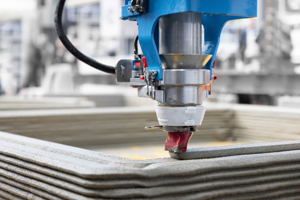
\includegraphics[width=0.85\columnwidth]{3dcp_printer.jpg}
    \caption{3D Concrete Printer at the NITK Surathkal 3DCP Laboratory.}
    \label{fig:printer}
\end{figure}

\begin{figure}[t]
    \centering
    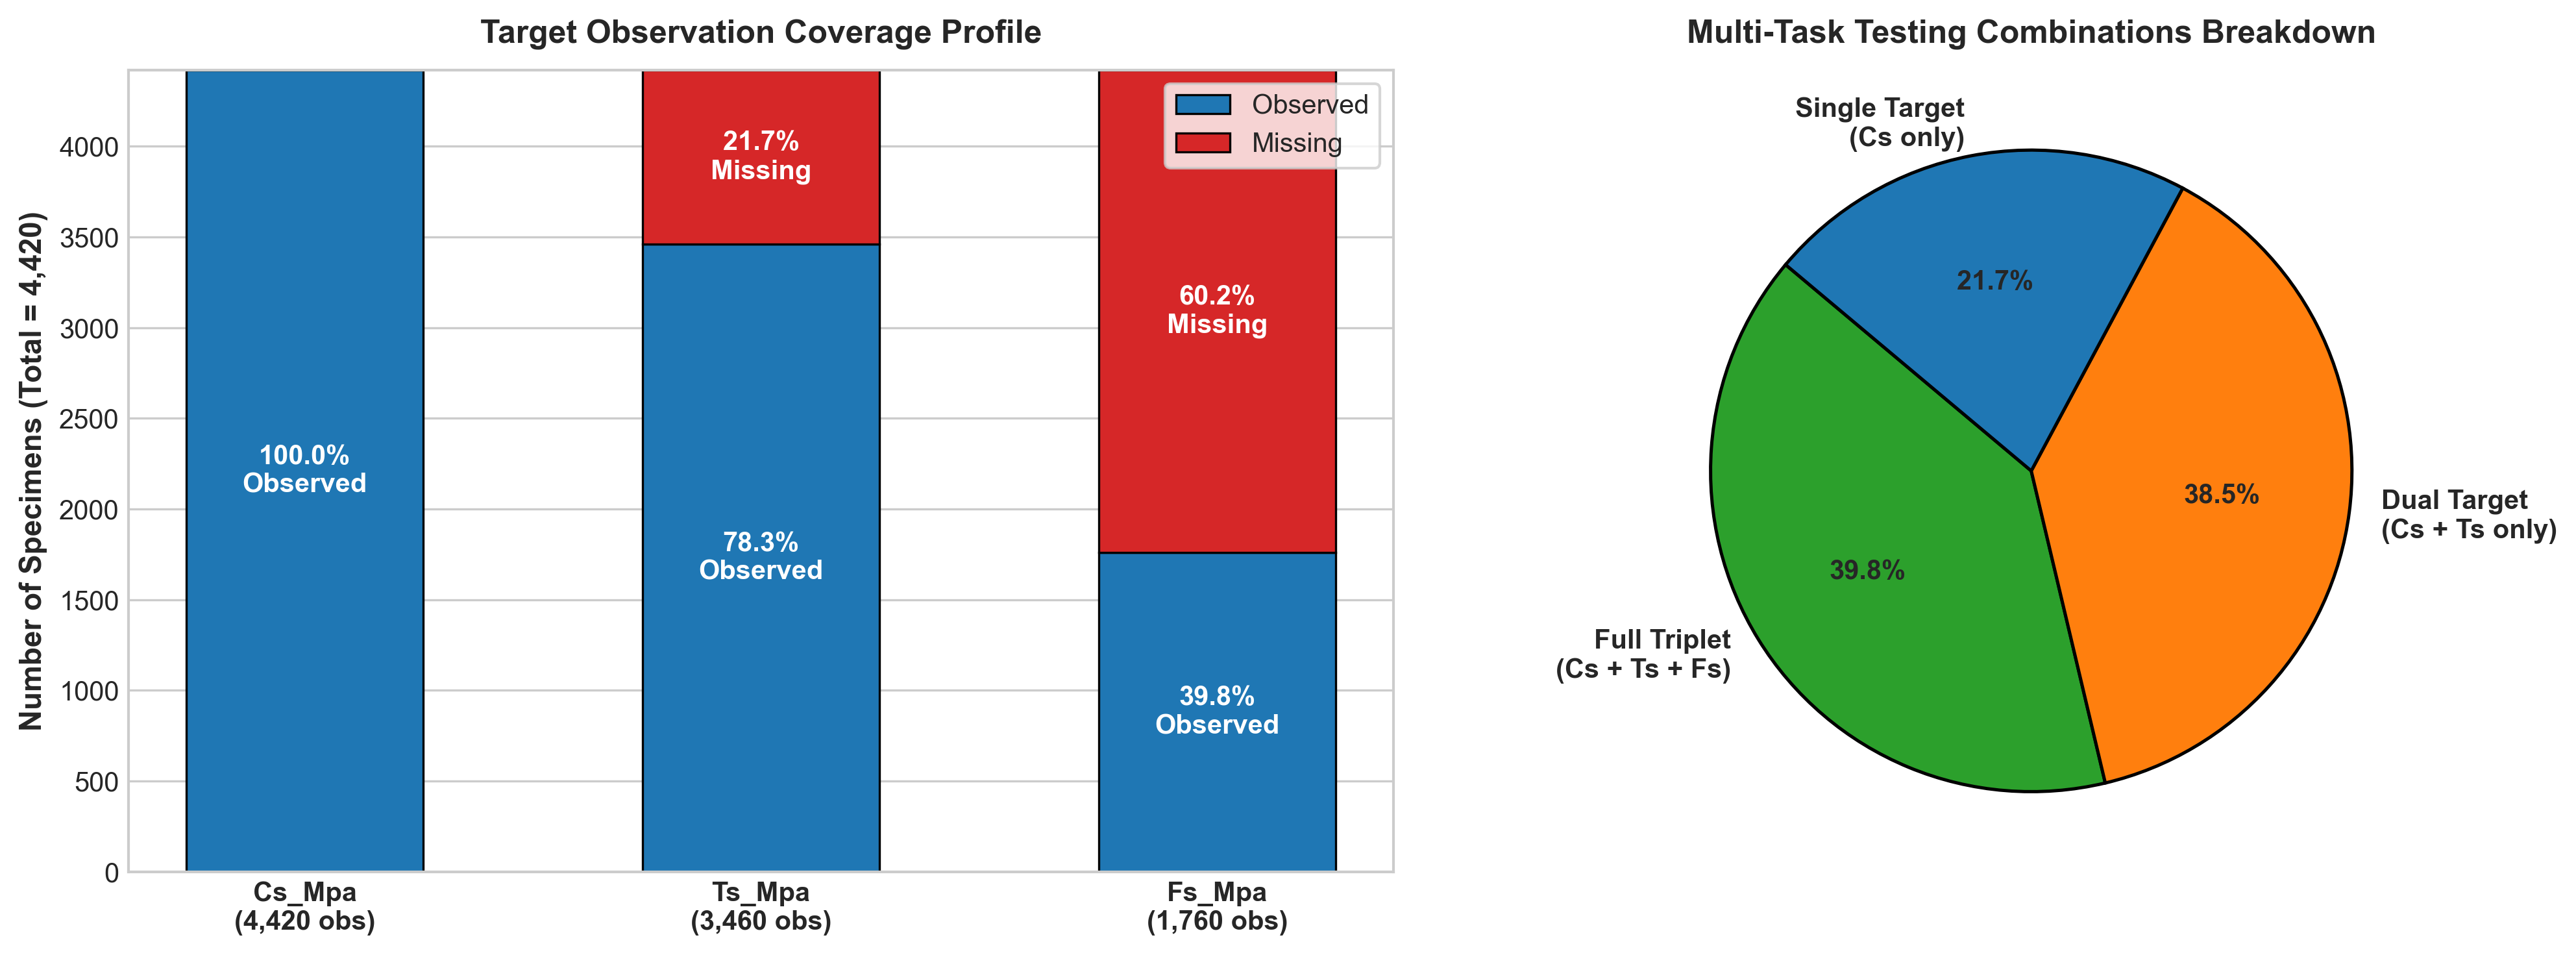
\includegraphics[width=\columnwidth]{01_target_missingness_profile.png}
    \caption{Target observation and asymmetric missingness profile across the 4,420 experimental mixes in the ConcreteXAI benchmark dataset.}
    \label{fig:missingness_profile}
\end{figure}

Consequently, real-world multivariate concrete databases exhibit severe \textit{asymmetric missingness}. In the international ConcreteXAI benchmark database~\cite{guzman2024concretexai} comprising 4,420 multivariate specimens, compressive strength is 100\% complete, but splitting tensile strength is missing in 21.7\% of specimens ($N = 960$), and flexural strength is missing in 60.2\% ($N = 2,660$). As shown in Fig.~\ref{fig:missingness_profile}, only 1,760 out of 4,420 mixes (39.8\%) possess complete three-property labels.

Standard machine learning practices fail in this setting:
\begin{itemize}
    \item \textbf{Complete-Case Analysis (Row Dropping):} Discarding incomplete records discards 60.2\% (2,660 mixes) of experimental data, destroying statistical power and inducing severe laboratory selection bias.
    \item \textbf{Artificial Imputation:} Filling unobserved strengths with mean, median, or $k$-nearest neighbor values introduces synthetic artifacts that corrupt empirical gradients.
    \item \textbf{Independent Single-Task Regressors:} Training separate models for each property ignores the continuum mechanics coupling between compression, tension, and rupture.
    \item \textbf{Unconstrained Neural Networks:} Standard multi-task networks frequently produce physically absurd outputs, predicting negative strengths, tensile capacities exceeding compressive strength ($T_s \ge C_s$), or out-of-code ratios.
\end{itemize}

To overcome these fundamental limitations, this work develops a \textbf{Physics-Informed Masked Multi-Task Learning (PIM-MTL)} architecture. The primary contributions of this paper are:
\begin{enumerate}
    \item \textbf{Masked Multi-Task Gradient Gating:} A unified multi-task loss formulation that enables training on all 4,420 mixes simultaneously. A binary observation mask ensures that unobserved targets receive strictly zero backpropagation gradient, utilizing 100\% of the data without synthetic imputation.
    \item \textbf{Differentiable Continuum Physics Regularization:} Embedding ACI 318 and Eurocode 2 ratio bounds ($0.06 \le T_s/C_s \le 0.18$ and $0.08 \le F_s/C_s \le 0.25$) directly into the PyTorch optimization graph via a two-sided quadratic hinge penalty evaluated on all specimens, regularizing unobserved heads via microstructural mechanics.
    \item \textbf{Production-Grade Deployment Architecture:} Incorporating a custom \texttt{SafeBatchNorm1d} layer that eliminates runtime exceptions during single-specimen ($N=1$) on-site inference, combined with Gaussian Error Linear Units (GELU) and Cosine Annealing optimization.
    \item \textbf{Rigorous Quantitative and Physical Validation:} Demonstrating high predictive performance ($R^2 > 0.98$ on all targets), auditing five supervised baseline architectures (Ridge, Naive Bayes, XGBoost, LightGBM, Single-Task ANN), and verifying a 0.00\% rate of physically impossible predictions ($T_s \ge C_s$) across a standardized 1,326-sample held-out test split (30\% partition).
\end{enumerate}

\section{Related Work}

\subsection{Machine Learning in Concrete and 3DCP}
Recent literature has increasingly explored data-driven methods for concrete property prediction. Ali et al.~\cite{ali2023machine} investigated Support Vector Machines (SVM) and XGBoost regression to predict the tensile and flexural strength of 3D-printed concrete from mix formulations. Zhang et al.~\cite{zhang2025research} examined Random Forests and Artificial Neural Networks (ANN) for mechanical strength estimation, noting strong correlations with binder composition. Similarly, Feng et al.~\cite{feng2021machine} synthesized an extensive international database to assess compressive capacity. However, these prior studies treated strength prediction as isolated single-target regression tasks on complete datasets, discarding unobserved targets and neglecting multi-property mechanics.

\subsection{Multi-Task Learning and Incomplete Supervision}
Multi-Task Learning (MTL)~\cite{caruana1997multitask} aims to improve generalization by sharing representations across related tasks. In concrete mechanics, compressive, tensile, and flexural strengths originate from the same microstructural hydration products (calcium-silicate-hydrate gel, pore structure, and interfacial transition zone). Hence, an encoder trained on multiple targets should theoretically discover richer representations than disjoint models. However, classical MTL architectures assume complete target matrices. In sparse engineering datasets, naive masking often leads to gradient imbalance or vanishing updates. Developing exact gradient-gating mechanisms is crucial to maintain representation learning without distorting loss dynamics.

\subsection{Physics-Informed Neural Networks (PINN)}
Physics-informed machine learning, formalized by Karniadakis et al.~\cite{karniadakis2021physics}, integrates governing physical laws (such as partial differential equations, conservation principles, and empirical bounds) into deep neural loss functions. In structural concrete research, Feng et al.~\cite{feng2021machine} demonstrated that penalizing unphysical strength behaviors improves out-of-distribution robustness. In this paper, we extend physics regularization to multi-task learning under extreme missingness: by evaluating continuum ratio constraints on \textit{all} samples, the physical regularizer provides meaningful gradient guidance to unobserved prediction heads even in the total absence of ground-truth laboratory measurements.

\section{Problem Formulation and Mechanical Constraints}

\subsection{Mathematical Problem Setting}
Let $\mathcal{D} = \{(\mathbf{x}_i, \mathbf{y}_i, \mathbf{m}_i)\}_{i=1}^N$ denote a multivariate concrete dataset of $N = 4,420$ specimens.
Each input vector $\mathbf{x}_i \in \mathbb{R}^D$ comprises material composition, non-destructive test measurements, and curing age.
The target vector is defined as:
\begin{equation}
    \mathbf{y}_i = \begin{bmatrix} C_{s,i} & T_{s,i} & F_{s,i} \end{bmatrix}^T \in \mathbb{R}^3
\end{equation}
where $C_{s,i}$, $T_{s,i}$, and $F_{s,i}$ represent compressive, splitting tensile, and flexural strengths in Megapascals (MPa).

Because experimental observations are incomplete, each sample is associated with a binary observation mask:
\begin{equation}
    \mathbf{m}_i = \begin{bmatrix} m_{i,1} & m_{i,2} & m_{i,3} \end{bmatrix}^T \in \{0, 1\}^3
\end{equation}
where $m_{i,j} = 1$ if target $j$ was experimentally measured for specimen $i$, and $m_{i,j} = 0$ if the target is unobserved. For unobserved entries, a computational placeholder $y_{i,j} = 0.0$ is assigned in memory. The objective is to learn a parameter-shared neural network $\hat{\mathbf{y}}_i = f_\theta(\mathbf{x}_i)$ that accurately predicts all three mechanical properties while strictly respecting physical continuum bounds.

\subsection{Continuum Mechanics and Civil Engineering Code Envelopes}
Concrete is a quasi-brittle composite material whose tensile fracture is governed by microcrack propagation through the Interfacial Transition Zone (ITZ). Over a century of empirical testing and fracture mechanics formulations codified in ACI 318-19~\cite{aci318_19} and Eurocode 2~\cite{eurocode2} define strict physical relationships between compressive, tensile, and flexural strengths.

\subsubsection{Splitting Tensile to Compressive Ratio ($R_t$)}
According to ACI 318 Section 19.2.4 and Eurocode 2 Section 3.1.2, direct and splitting tensile capacities scale with the square root of compressive strength:
\begin{equation}
    f_{ct} \approx 0.53 \sqrt{f'_c} \quad \text{to} \quad 0.59 \sqrt{f'_c} \quad (\text{MPa})
\end{equation}
For typical concrete grades ($20 \le f'_c \le 55$~MPa), the theoretical ratio $R_t = T_s / C_s$ evaluates to approximately $0.08$ to $0.12$. Accounting for aggregate mineralogy, Blaine fineness, and chemical admixtures, standard compliant structural concrete satisfies the envelope:
\begin{equation}
    0.06 \le R_t = \frac{T_s}{C_s} \le 0.18
\end{equation}
A ratio below $0.06$ signifies severe matrix delamination, while a ratio exceeding $0.18$ violates the Mohr-Coulomb failure criterion for unreinforced cementitious paste. Moreover, sound concrete can never be stronger in tension than in compression; thus, $T_s < C_s$ is a mandatory physical invariant ($R_t < 1.0$).

\subsubsection{Flexural to Compressive Ratio ($R_f$)}
Flexural strength (Modulus of Rupture, $F_s$) evaluates extreme fiber bending capacity (ASTM C78~\cite{astm_c78}). Standard codes specify:
\begin{equation}
    f_r \approx 0.62 \sqrt{f'_c} \quad \text{to} \quad 0.83 \sqrt{f'_c} \quad (\text{MPa})
\end{equation}
which defines the physical envelope:
\begin{equation}
    0.08 \le R_f = \frac{F_s}{C_s} \le 0.25
\end{equation}

\subsubsection{Hierarchy Between Flexural and Tensile Capacity}
In third-point bending, peak tensile stresses occur solely along the extreme outer fiber, whereas splitting tension subjects the entire diametral plane to tensile stress. Owing to Weibull's weakest-link volume effect and microplastic stress redistribution, apparent flexural strength is consistently higher than splitting tensile strength ($F_s > T_s$). Unconstrained regressors that violate this hierarchy produce structurally dangerous predictions.

\section{Dataset Description and Exploratory Analysis}

\subsection{ConcreteXAI Benchmark Overview}
This investigation utilizes the 4,420 multivariate concrete specimen records from the benchmark ConcreteXAI database~\cite{guzman2024concretexai}. The dataset incorporates four categorical mix design parameters and four continuous predictors:
\begin{itemize}
    \item \texttt{Type\_of\_cement} (4 levels: CPC 30R, CPO 30R RS BRA, CPC 30R RS, CPC 40R): Dictates early vs. late calcium silicate hydrate ($C$-$S$-$H$) gel kinetics.
    \item \texttt{Brand} (2 levels: CEMEX [3,540 specimens], Apasco [880 specimens]): Captures manufacturer clinker fineness and gypsum balance.
    \item \texttt{Additives} (5 levels: None, Opuntia biopolymer, 10\% Blast Furnace Slag, Fluidizers): Modulates rheology and ITZ densification.
    \item \texttt{Type\_of\_aggregates} (4 levels: Crushed, Rounded gravel, Recycled concrete, Volcanic): Determines mechanical interlock and aggregate stiffness.
    \item \texttt{Design\_Fc\_Mpa} (Continuous, range $20.0 - 35.0$~MPa): Nominal 28-day target design strength.
    \item \texttt{Curing\_age\_days} (Continuous, range $7 - 120$~days): Moist curing maturity.
    \item \texttt{Er\_ohm-cm} (Continuous, range $1.43 - 23.95~\Omega\cdot\text{cm}$): Bulk electrical resistivity, reflecting pore tortuosity and moisture content.
    \item \texttt{UPV\_m/s} (Continuous, range $2,431 - 5,319$~m/s): Ultrasonic Pulse Velocity, measuring ultrasonic transit speed and dynamic matrix density.
\end{itemize}

\begin{figure*}[t]
    \centering
    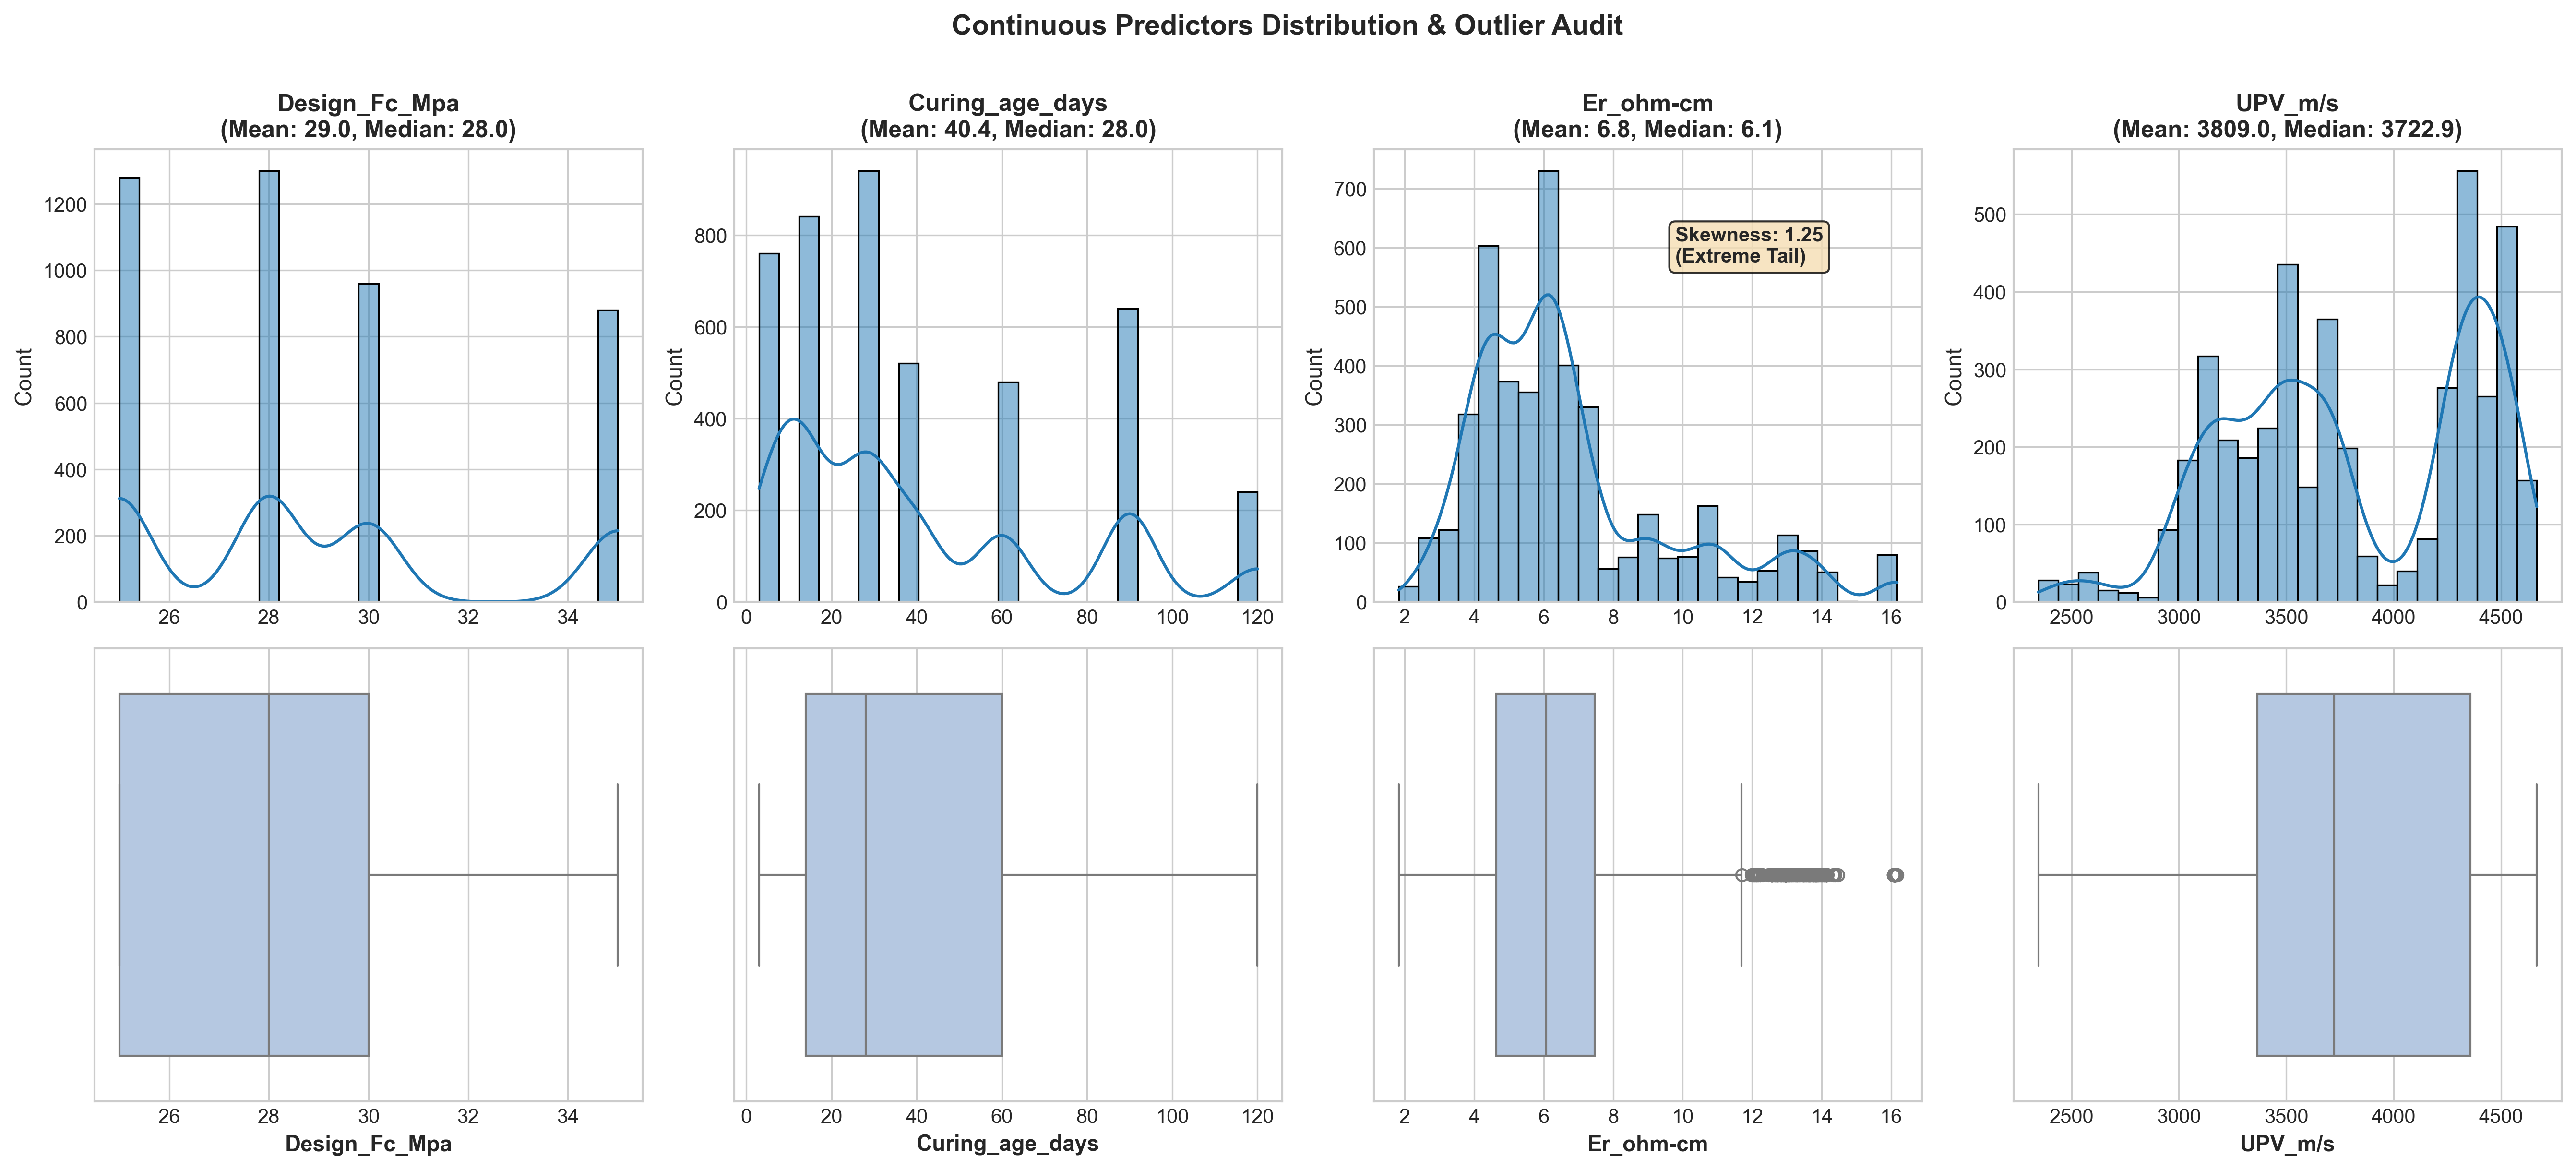
\includegraphics[width=0.95\textwidth]{02_continuous_features_distribution.png}
    \caption{Probability density distributions and boxplots of the continuous input features in the ConcreteXAI benchmark dataset.}
    \label{fig:continuous_dist}
\end{figure*}

\begin{figure}[t]
    \centering
    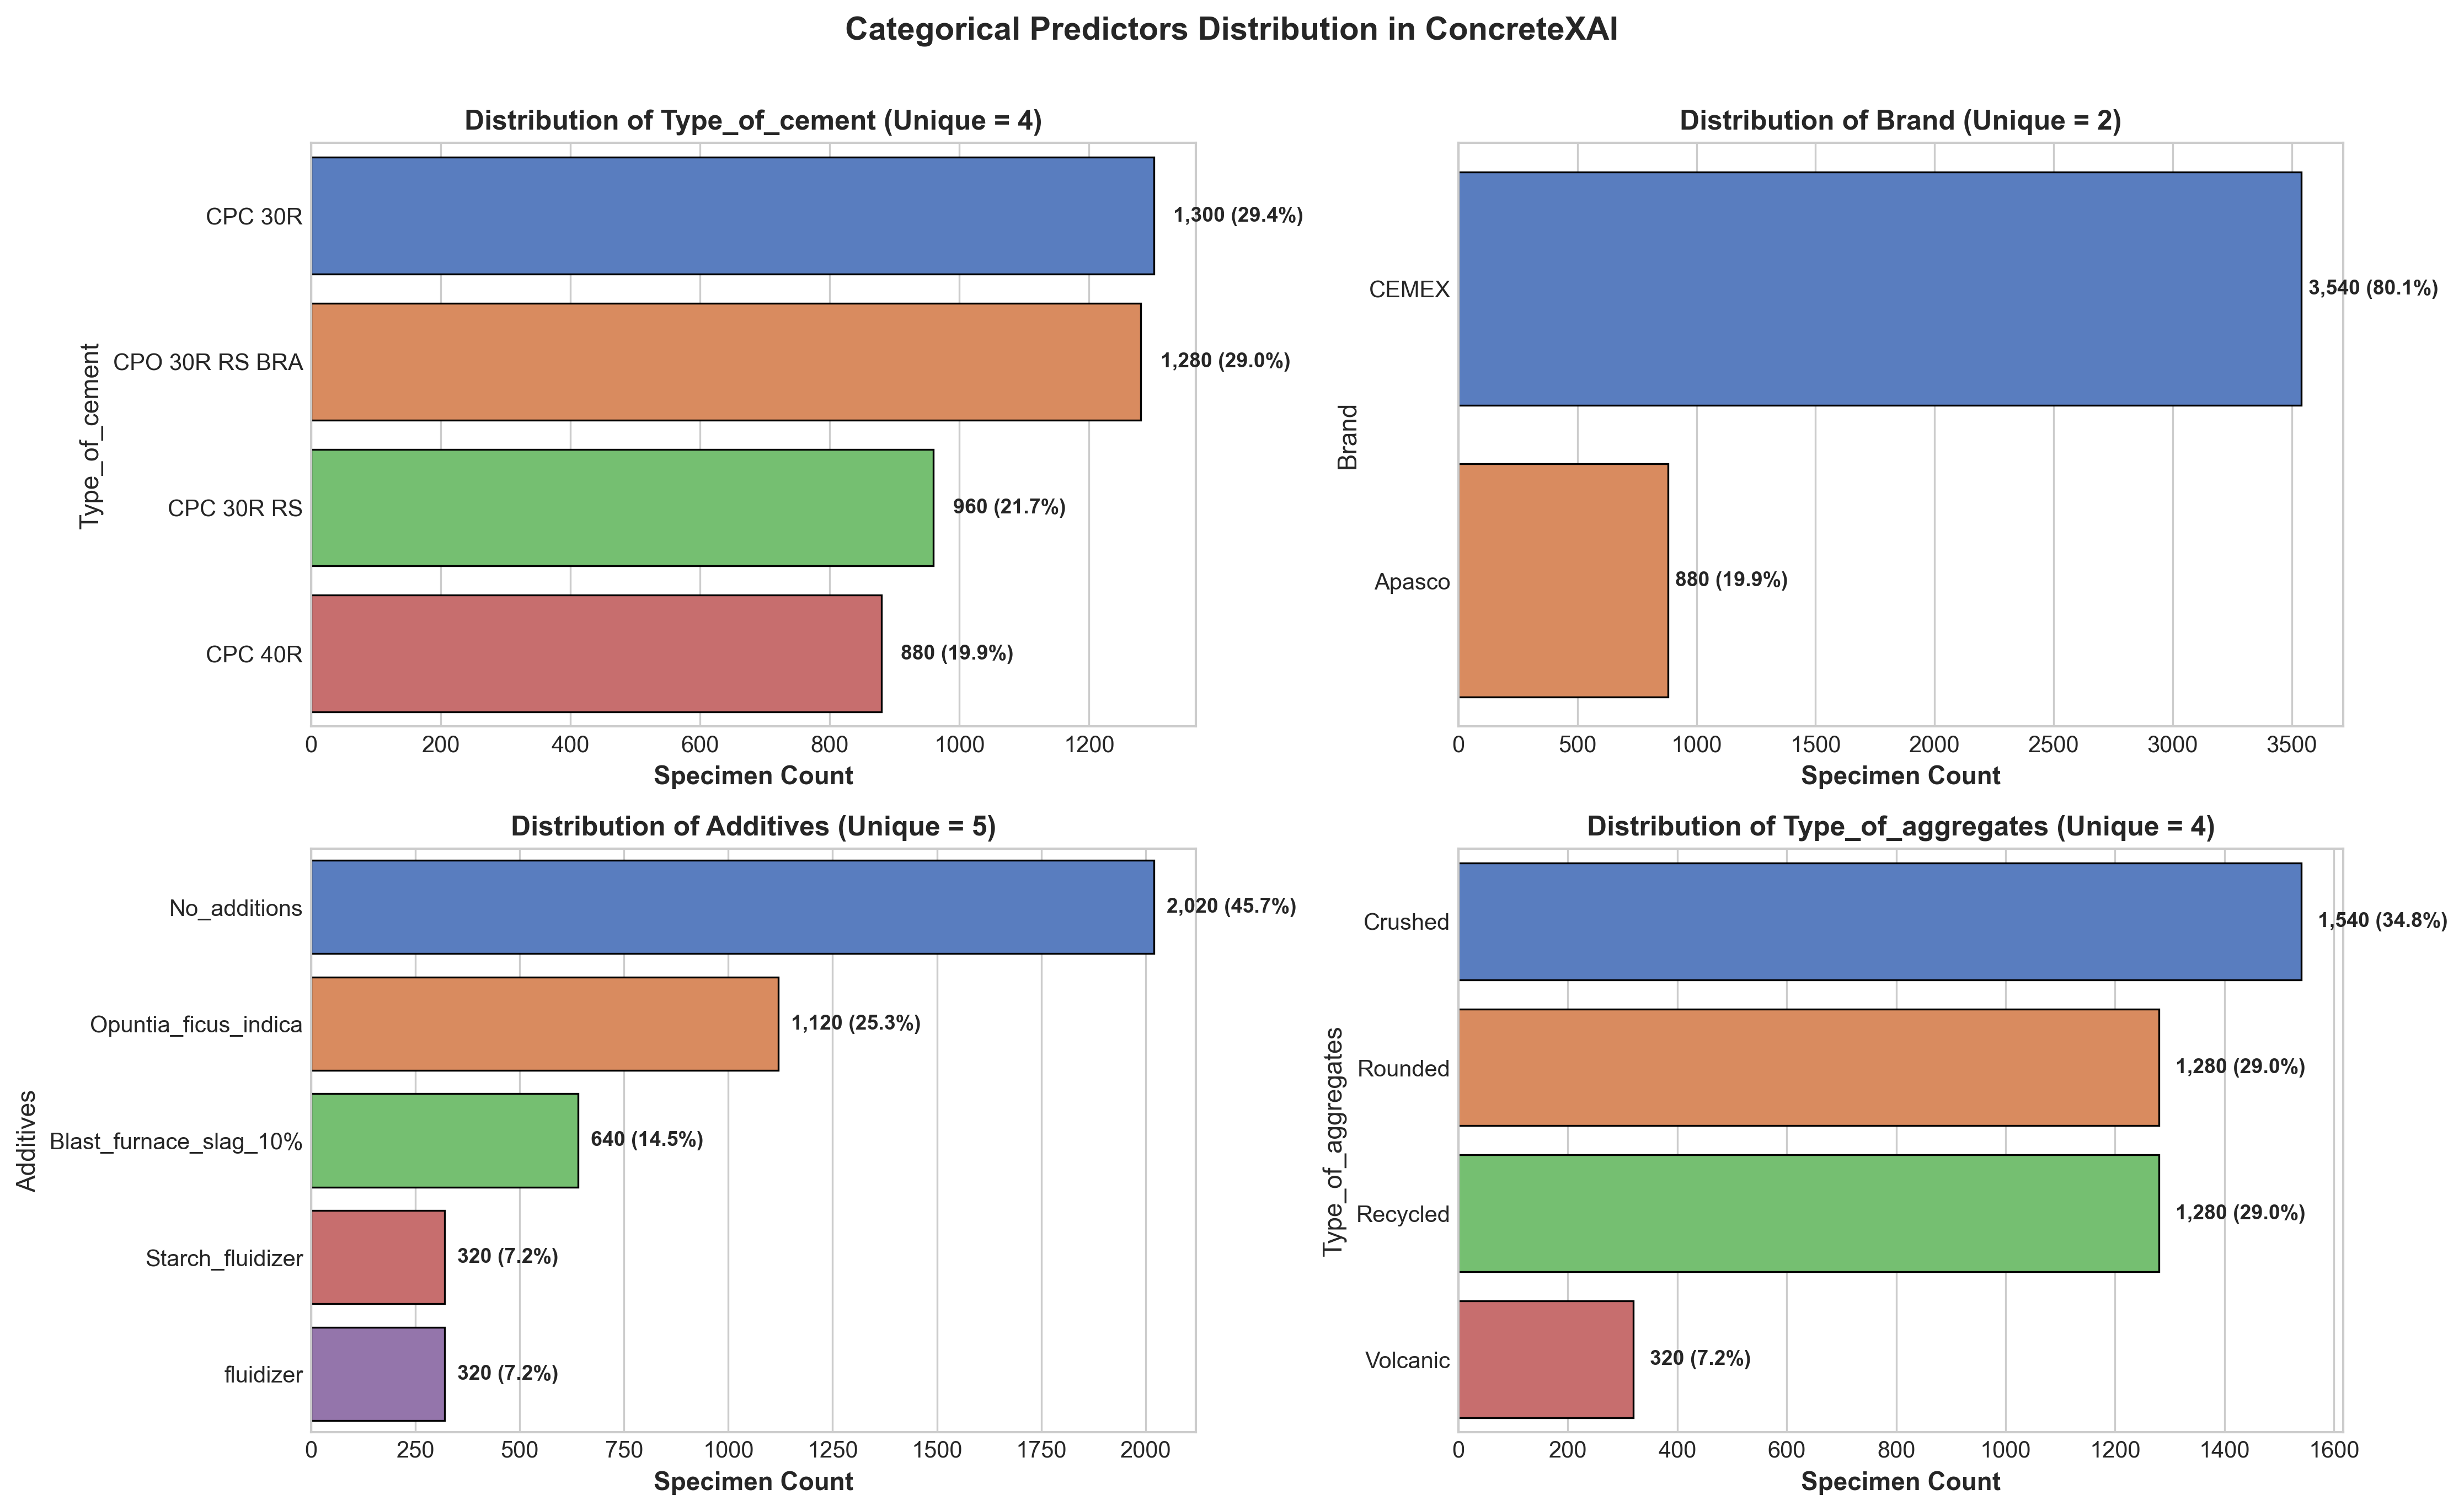
\includegraphics[width=\columnwidth]{03_categorical_features_distribution.png}
    \caption{Frequency distribution of categorical variables across mix specimens.}
    \label{fig:categorical_dist}
\end{figure}

\begin{figure*}[t]
    \centering
    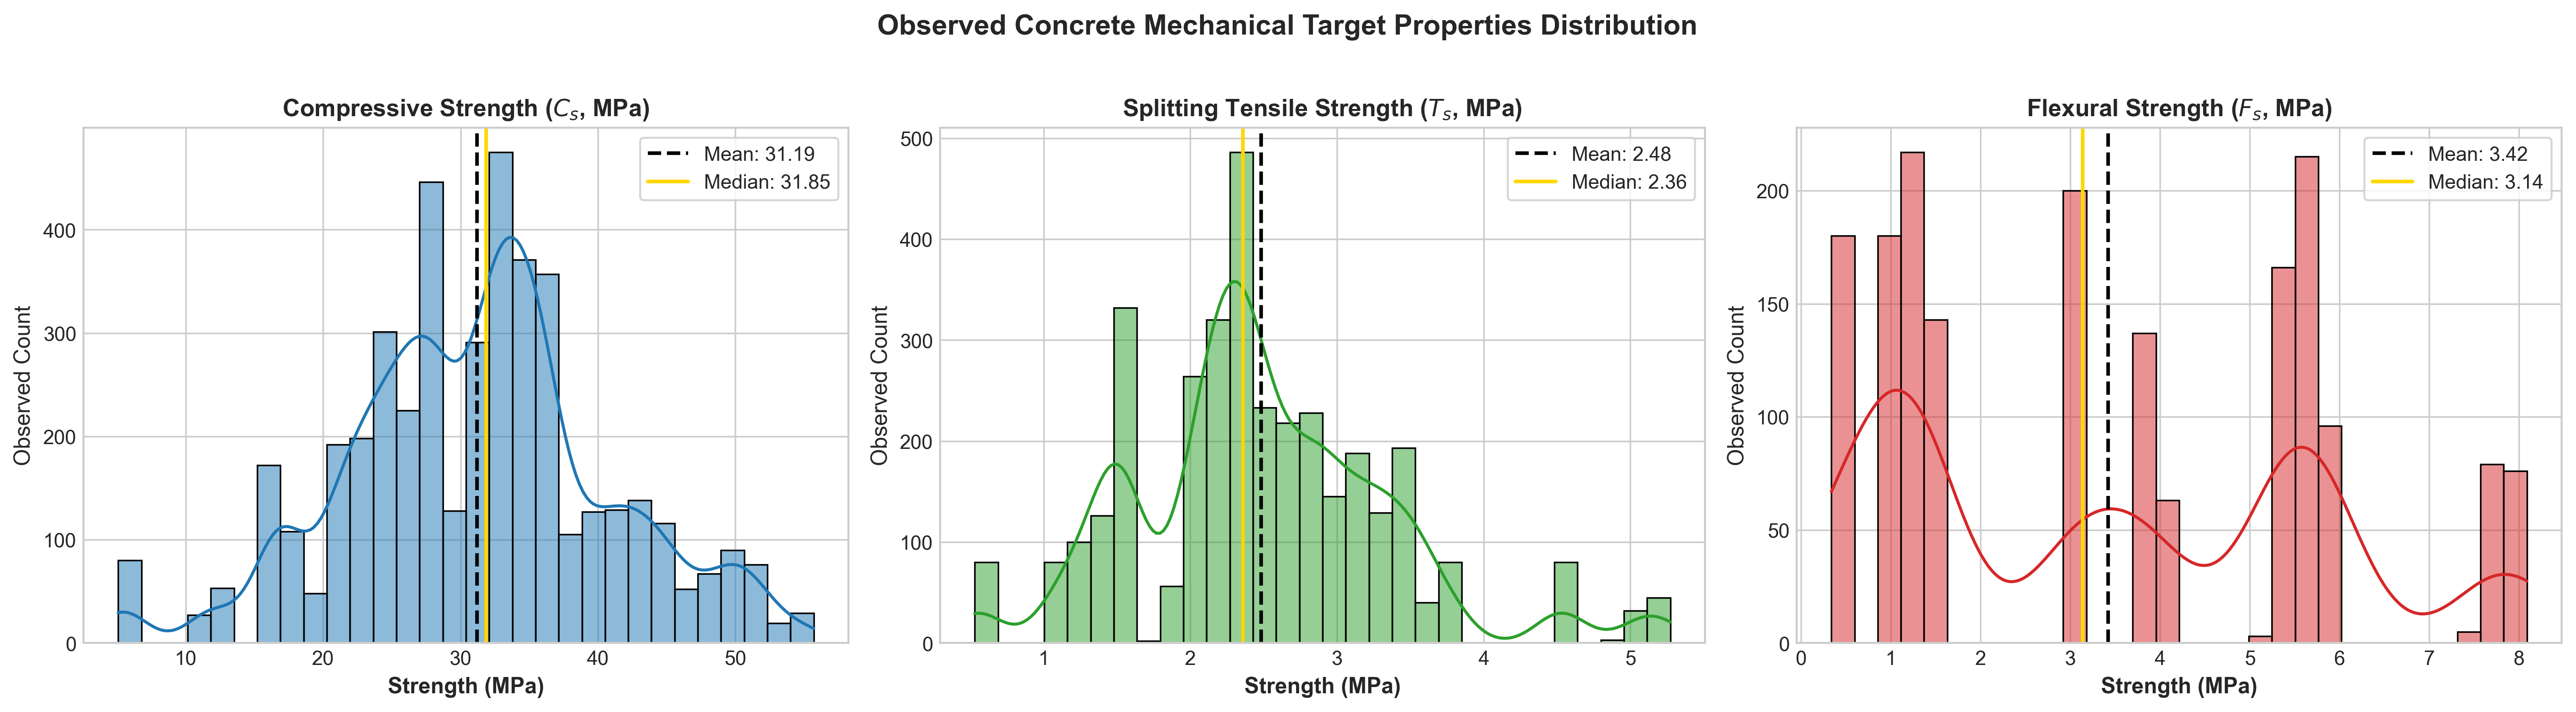
\includegraphics[width=0.95\textwidth]{04_target_distributions.png}
    \caption{Empirical probability distributions, kernel density estimations, and summary statistics of the three mechanical target variables.}
    \label{fig:target_dist}
\end{figure*}

\begin{figure}[t]
    \centering
    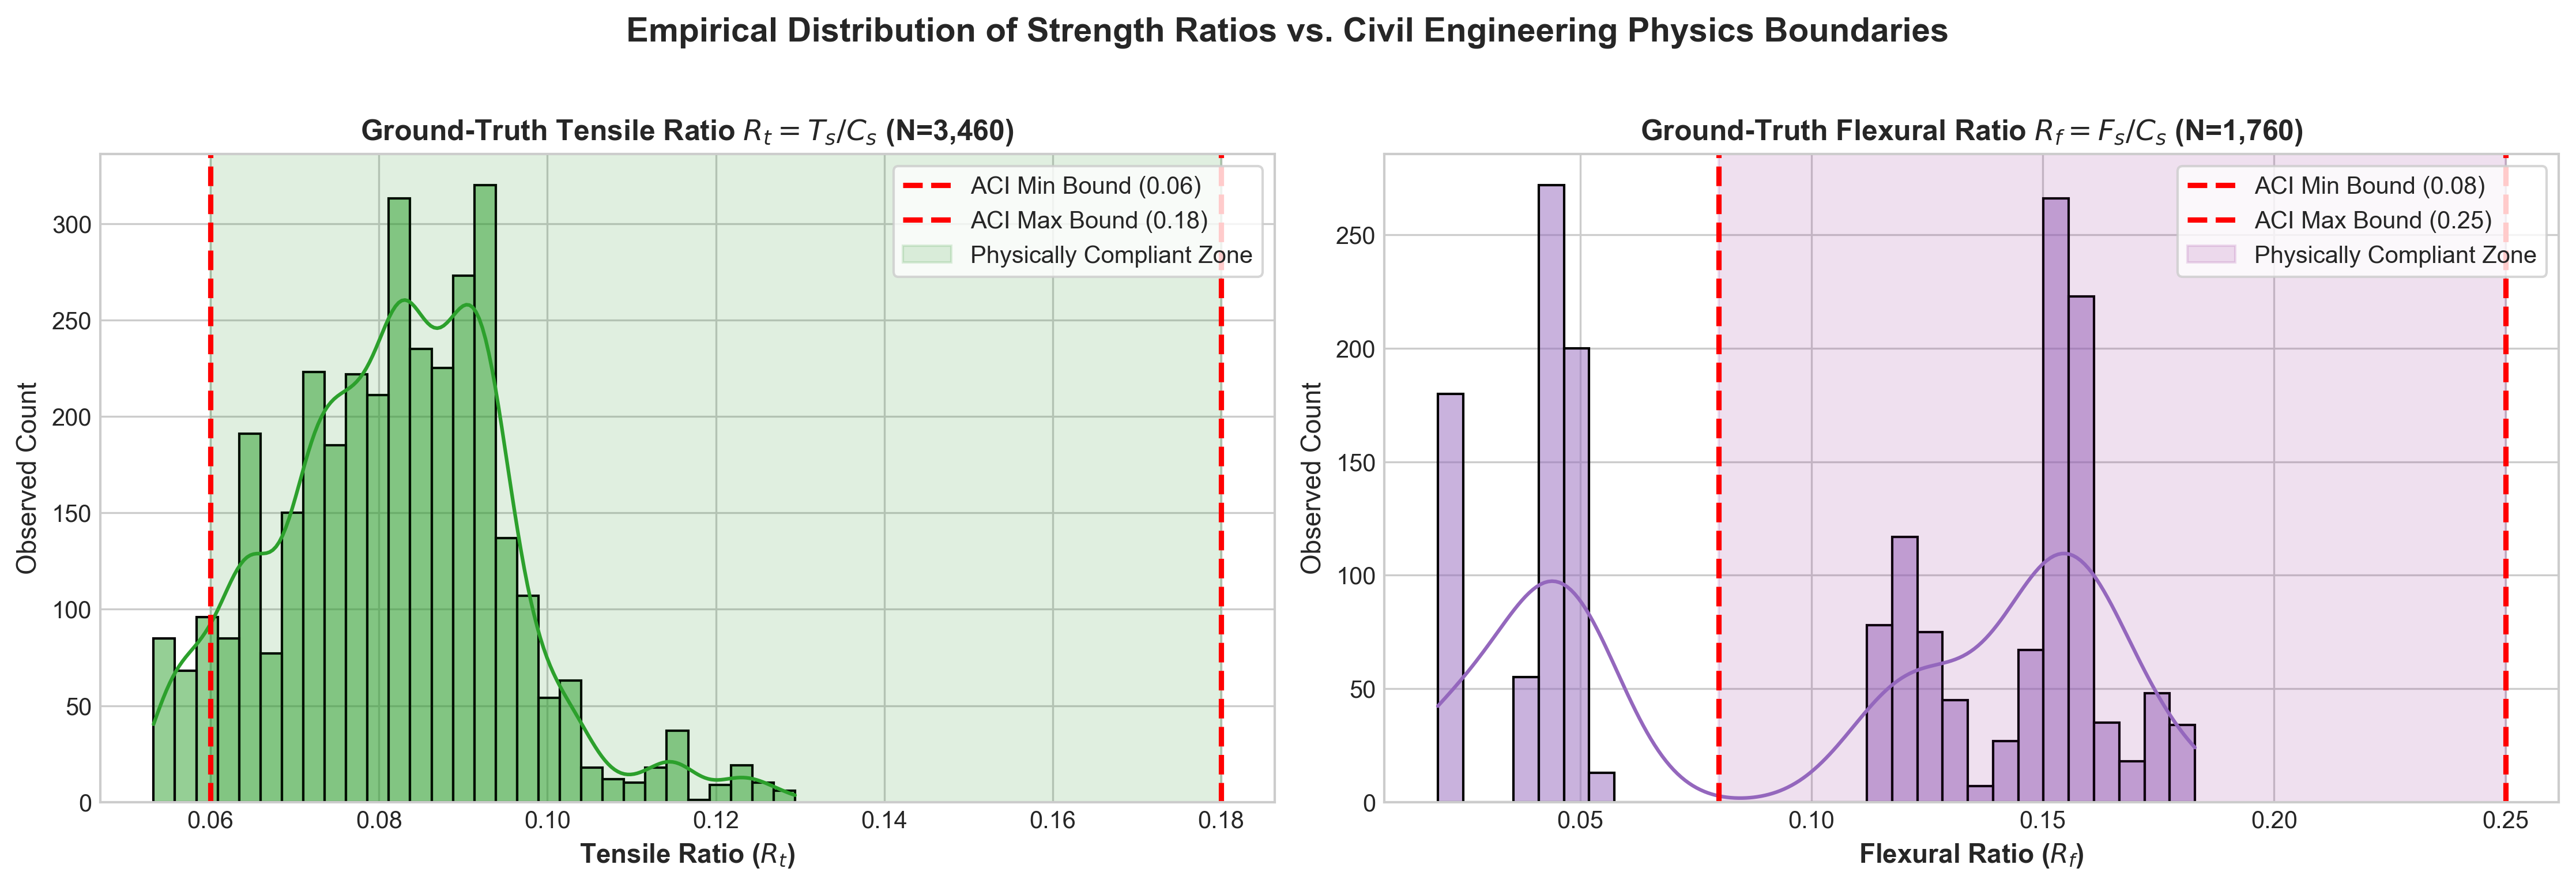
\includegraphics[width=\columnwidth]{05_ground_truth_mechanical_ratios.png}
    \caption{Ground truth mechanical ratio distributions ($T_s/C_s$ and $F_s/C_s$) overlaid with ACI 318 / Eurocode 2 theoretical boundary limits.}
    \label{fig:ground_truth_ratios}
\end{figure}

\begin{figure}[t]
    \centering
    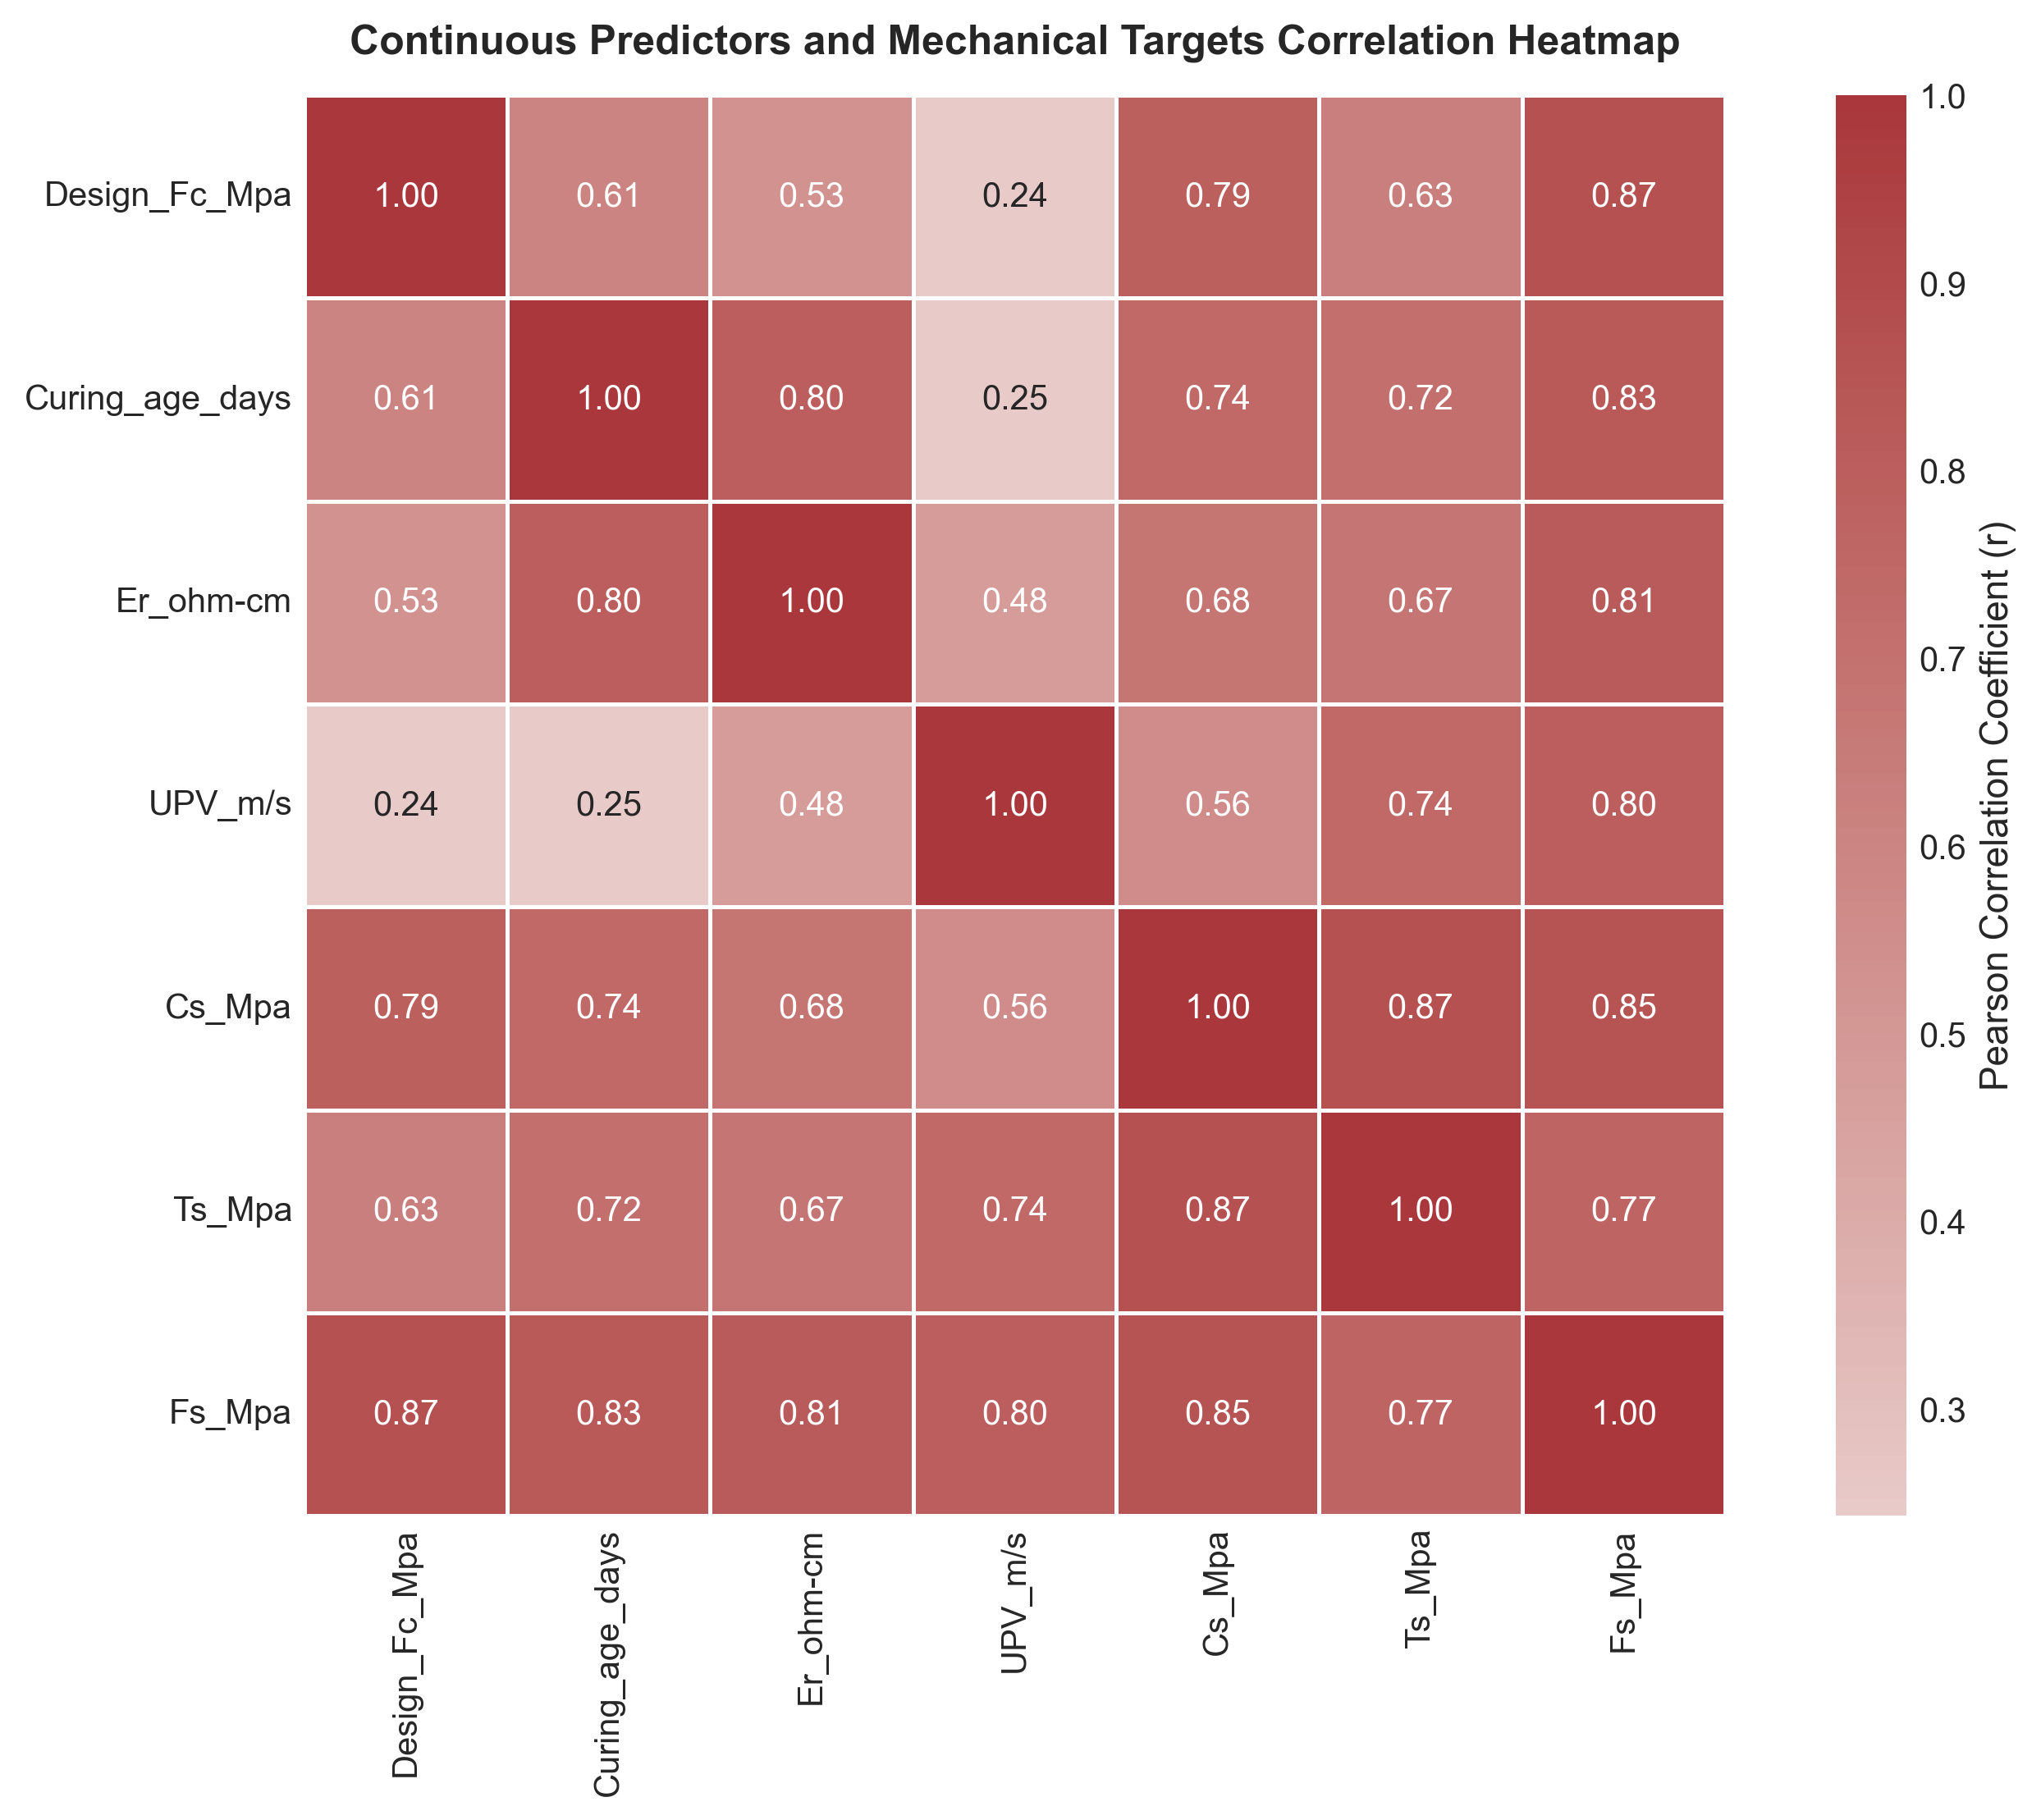
\includegraphics[width=\columnwidth]{06_correlation_matrix.png}
    \caption{Pearson correlation matrix between continuous features and target mechanical properties.}
    \label{fig:correlation_matrix}
\end{figure}

\subsection{Distributions and Mechanical Ratio Verification}
Fig.~\ref{fig:continuous_dist} illustrates the distributions of continuous features. Electrical resistivity exhibits marked positive skewness, with localized high-resistivity outliers indicative of advanced matrix desiccation. Fig.~\ref{fig:categorical_dist} summarizes categorical class frequencies, showing a dominant representation of CEMEX brand cements and diverse aggregate types.

The three target distributions are detailed in Fig.~\ref{fig:target_dist}:
\begin{itemize}
    \item \textbf{$C_s$ (`Cs\_Mpa`):} $N=4,420$ (100\% complete), Mean = $31.19 \pm 7.91$~MPa, Range = $[9.07, 55.71]$~MPa.
    \item \textbf{$T_s$ (`Ts\_Mpa`):} $N=3,460$ (78.3\% observed), Mean = $2.48 \pm 0.65$~MPa, Range = $[0.78, 5.27]$~MPa.
    \item \textbf{$F_s$ (`Fs\_Mpa`):} $N=1,760$ (39.8\% observed), Mean = $3.42 \pm 1.34$~MPa, Range = $[0.29, 8.09]$~MPa.
\end{itemize}

Crucially, Fig.~\ref{fig:ground_truth_ratios} plots the empirical ratio distributions of observed specimens against theoretical code bounds. For splitting tensile strength, 96.8\% of ground-truth mixes fall within the ACI 318 envelope ($0.06 \le R_t \le 0.18$). For flexural strength, the empirical distribution centers around $0.11$, with 82.2\% strictly inside $[0.08, 0.25]$. This confirms that real experimental mixes adhere to continuum mechanical ratio bounds, providing strong empirical justification for our physics loss formulation. Fig.~\ref{fig:correlation_matrix} displays the feature correlation matrix, highlighting strong positive coupling between non-destructive ultrasonic velocity (UPV) and compressive strength ($r = 0.74$).

\section{Proposed PIM-MTL Methodology}

The overall operational architecture of the proposed Physics-Informed Masked Multi-Task Learning (PIM-MTL) framework is depicted in Fig.~\ref{fig:system_workflow}. The system comprises an end-to-end pipeline structured across five primary stages: (1) multi-property tabular input ingestion, (2) strictly isolated preprocessing and binary mask generation, (3) deep shared-representation encoding and multi-task projection, (4) hybrid optimization coupling masked empirical loss with continuum physics regularization, and (5) persistent model and evaluation artifact export.

\begin{figure*}[t]
    \centering
    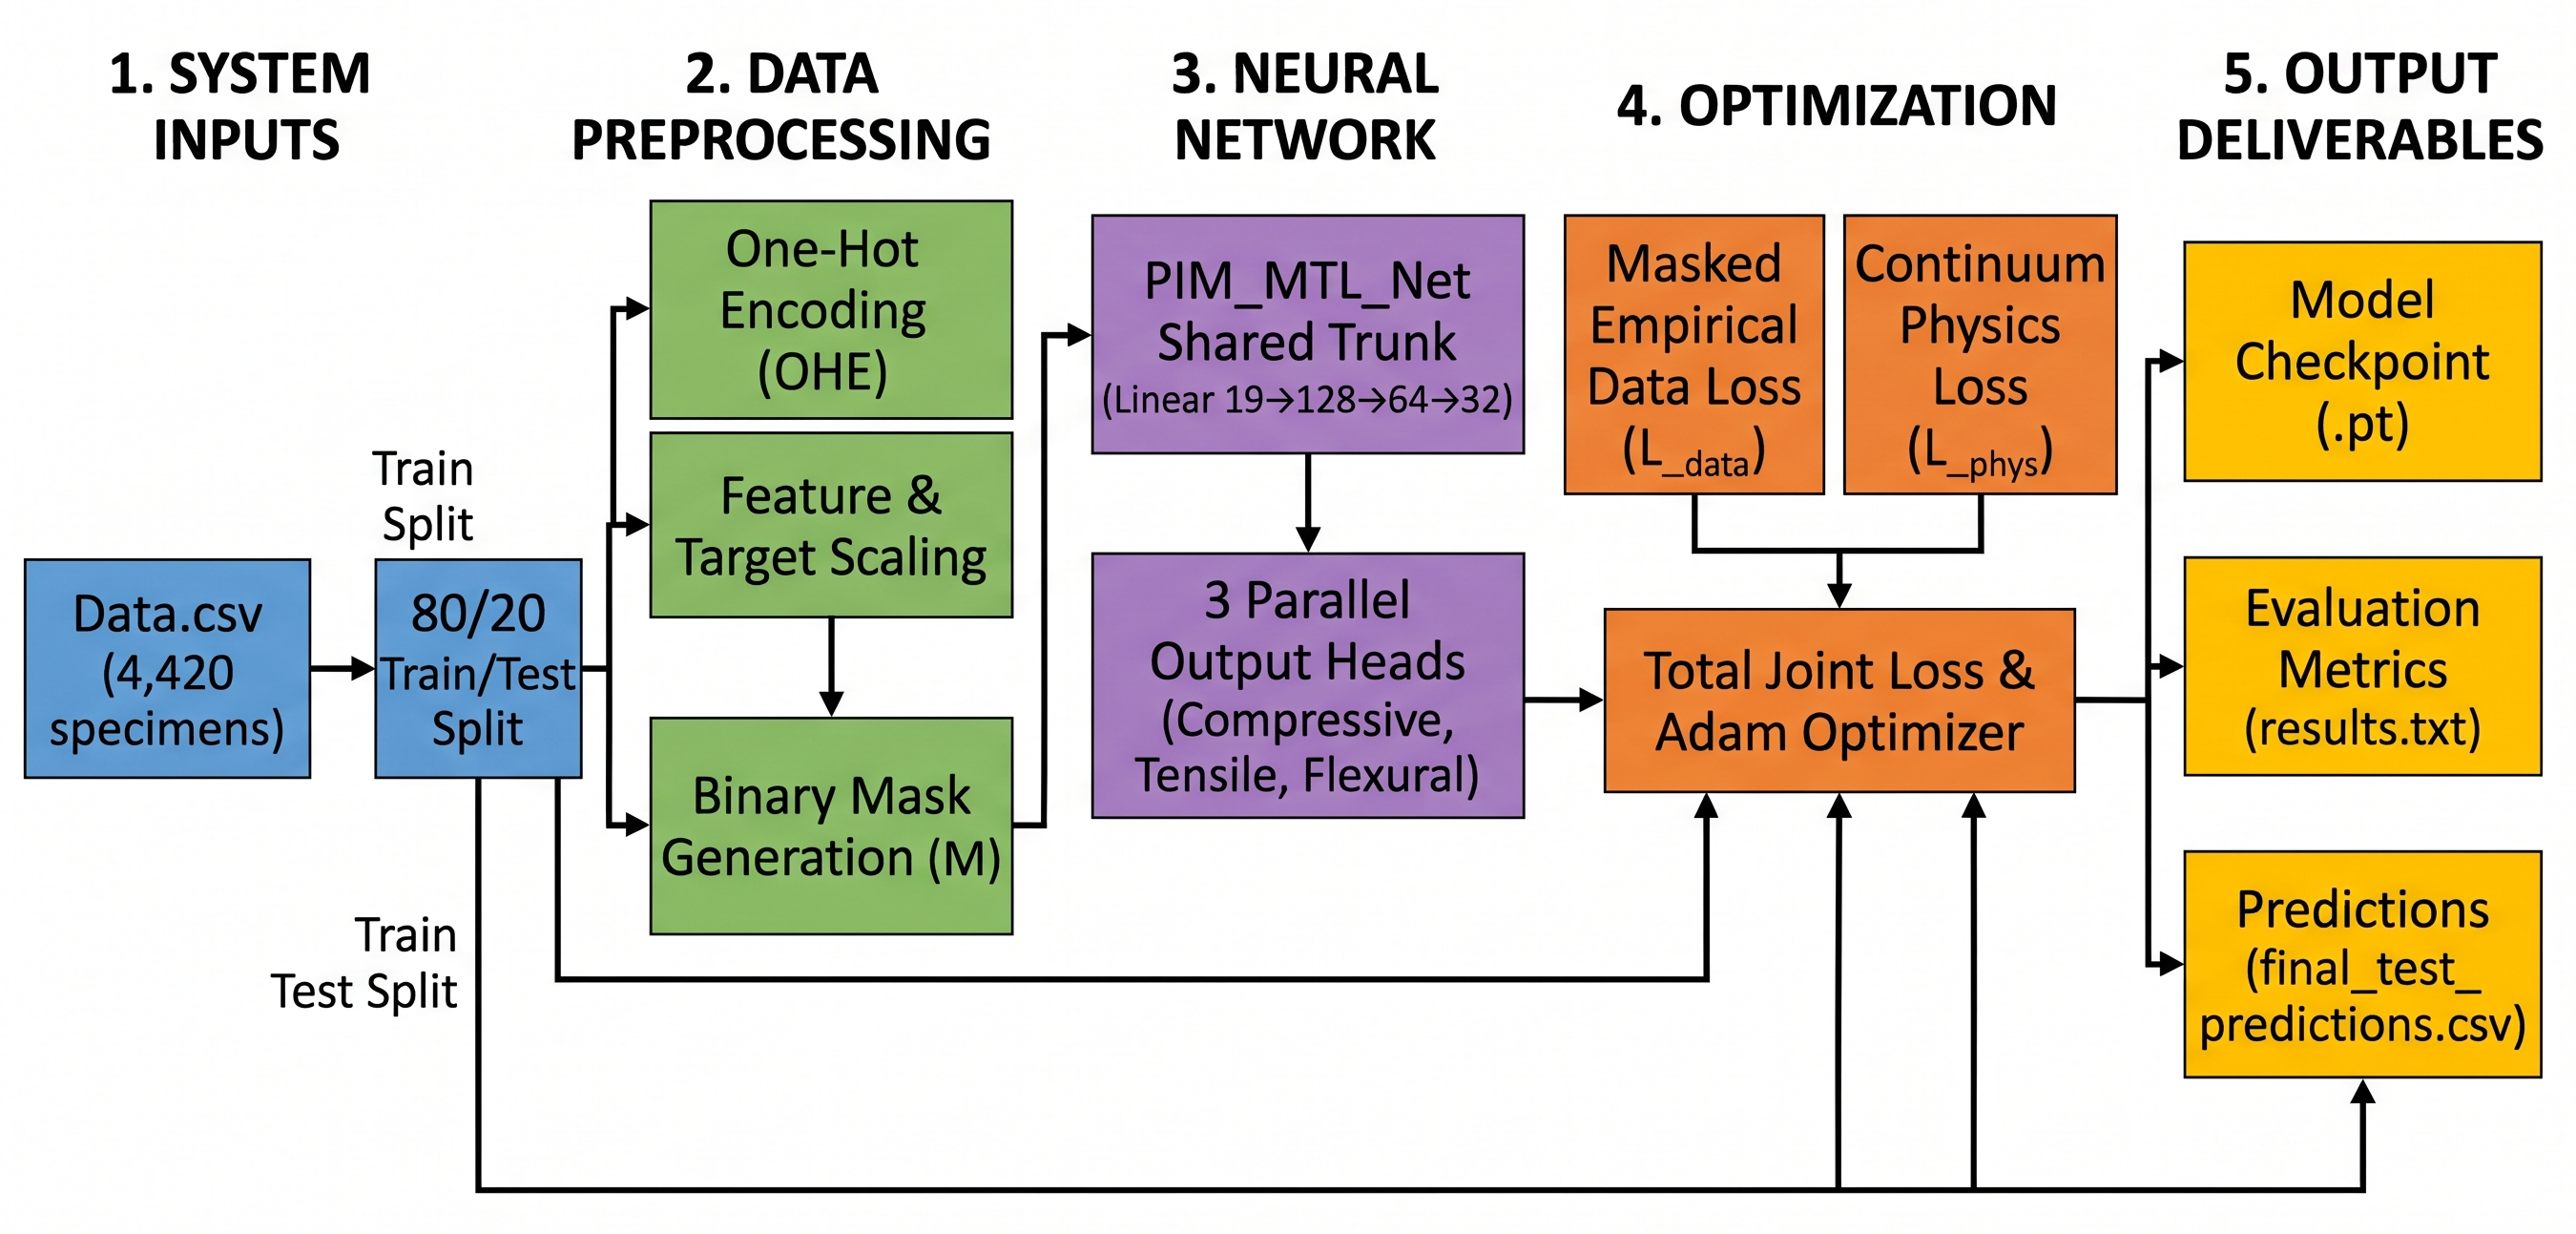
\includegraphics[width=0.96\textwidth]{workflow.png}
    \caption{End-to-end operational workflow of the proposed Physics-Informed Masked Multi-Task Learning (PIM-MTL) framework, detailing: (1) multi-property input ingestion, (2) leakage-free preprocessing with categorical encoding and binary mask generation, (3) shared representation neural network, (4) hybrid masked data and continuum physics optimization, and (5) persistent model and evaluation deliverables.}
    \label{fig:system_workflow}
\end{figure*}

\subsection{Leakage-Free Preprocessing Pipeline}
To ensure strict scientific integrity, all preprocessing transformers are fitted exclusively on the 70\% training partition ($N_{\text{train}} = 3,094$), leaving the 30\% held-out test partition ($N_{\text{test}} = 1,326$) completely isolated:
\begin{enumerate}
    \item \textbf{Categorical Encoding:} The 4 categorical variables are expanded into 15 binary indicators using \texttt{OneHotEncoder(handle\_unknown='ignore', sparse\_output=False)}.
    \item \textbf{Continuous Feature Scaling:} To mitigate the influence of skewed electrical resistivity values without distorting physical variance, continuous features are normalized via \texttt{RobustScaler}:
    \begin{equation}
        x_{\text{scaled}} = \frac{x - \text{median}(x_{\text{train}})}{\text{IQR}(x_{\text{train}})}
    \end{equation}
    where $\text{IQR} = Q_3 - Q_1$. Post-concatenation, the preprocessed input vector spans $D = 15 + 4 = 19$ dimensions.
    \item \textbf{Target Normalization:} Target scalers are fitted \textit{strictly on observed training instances} for each task. Unobserved target entries are filled with $0.0$ placeholders in the scaled matrix $\mathbf{Y}_{\text{scaled}} \in \mathbb{R}^{N \times 3}$.
\end{enumerate}

\begin{figure*}[t]
    \centering
    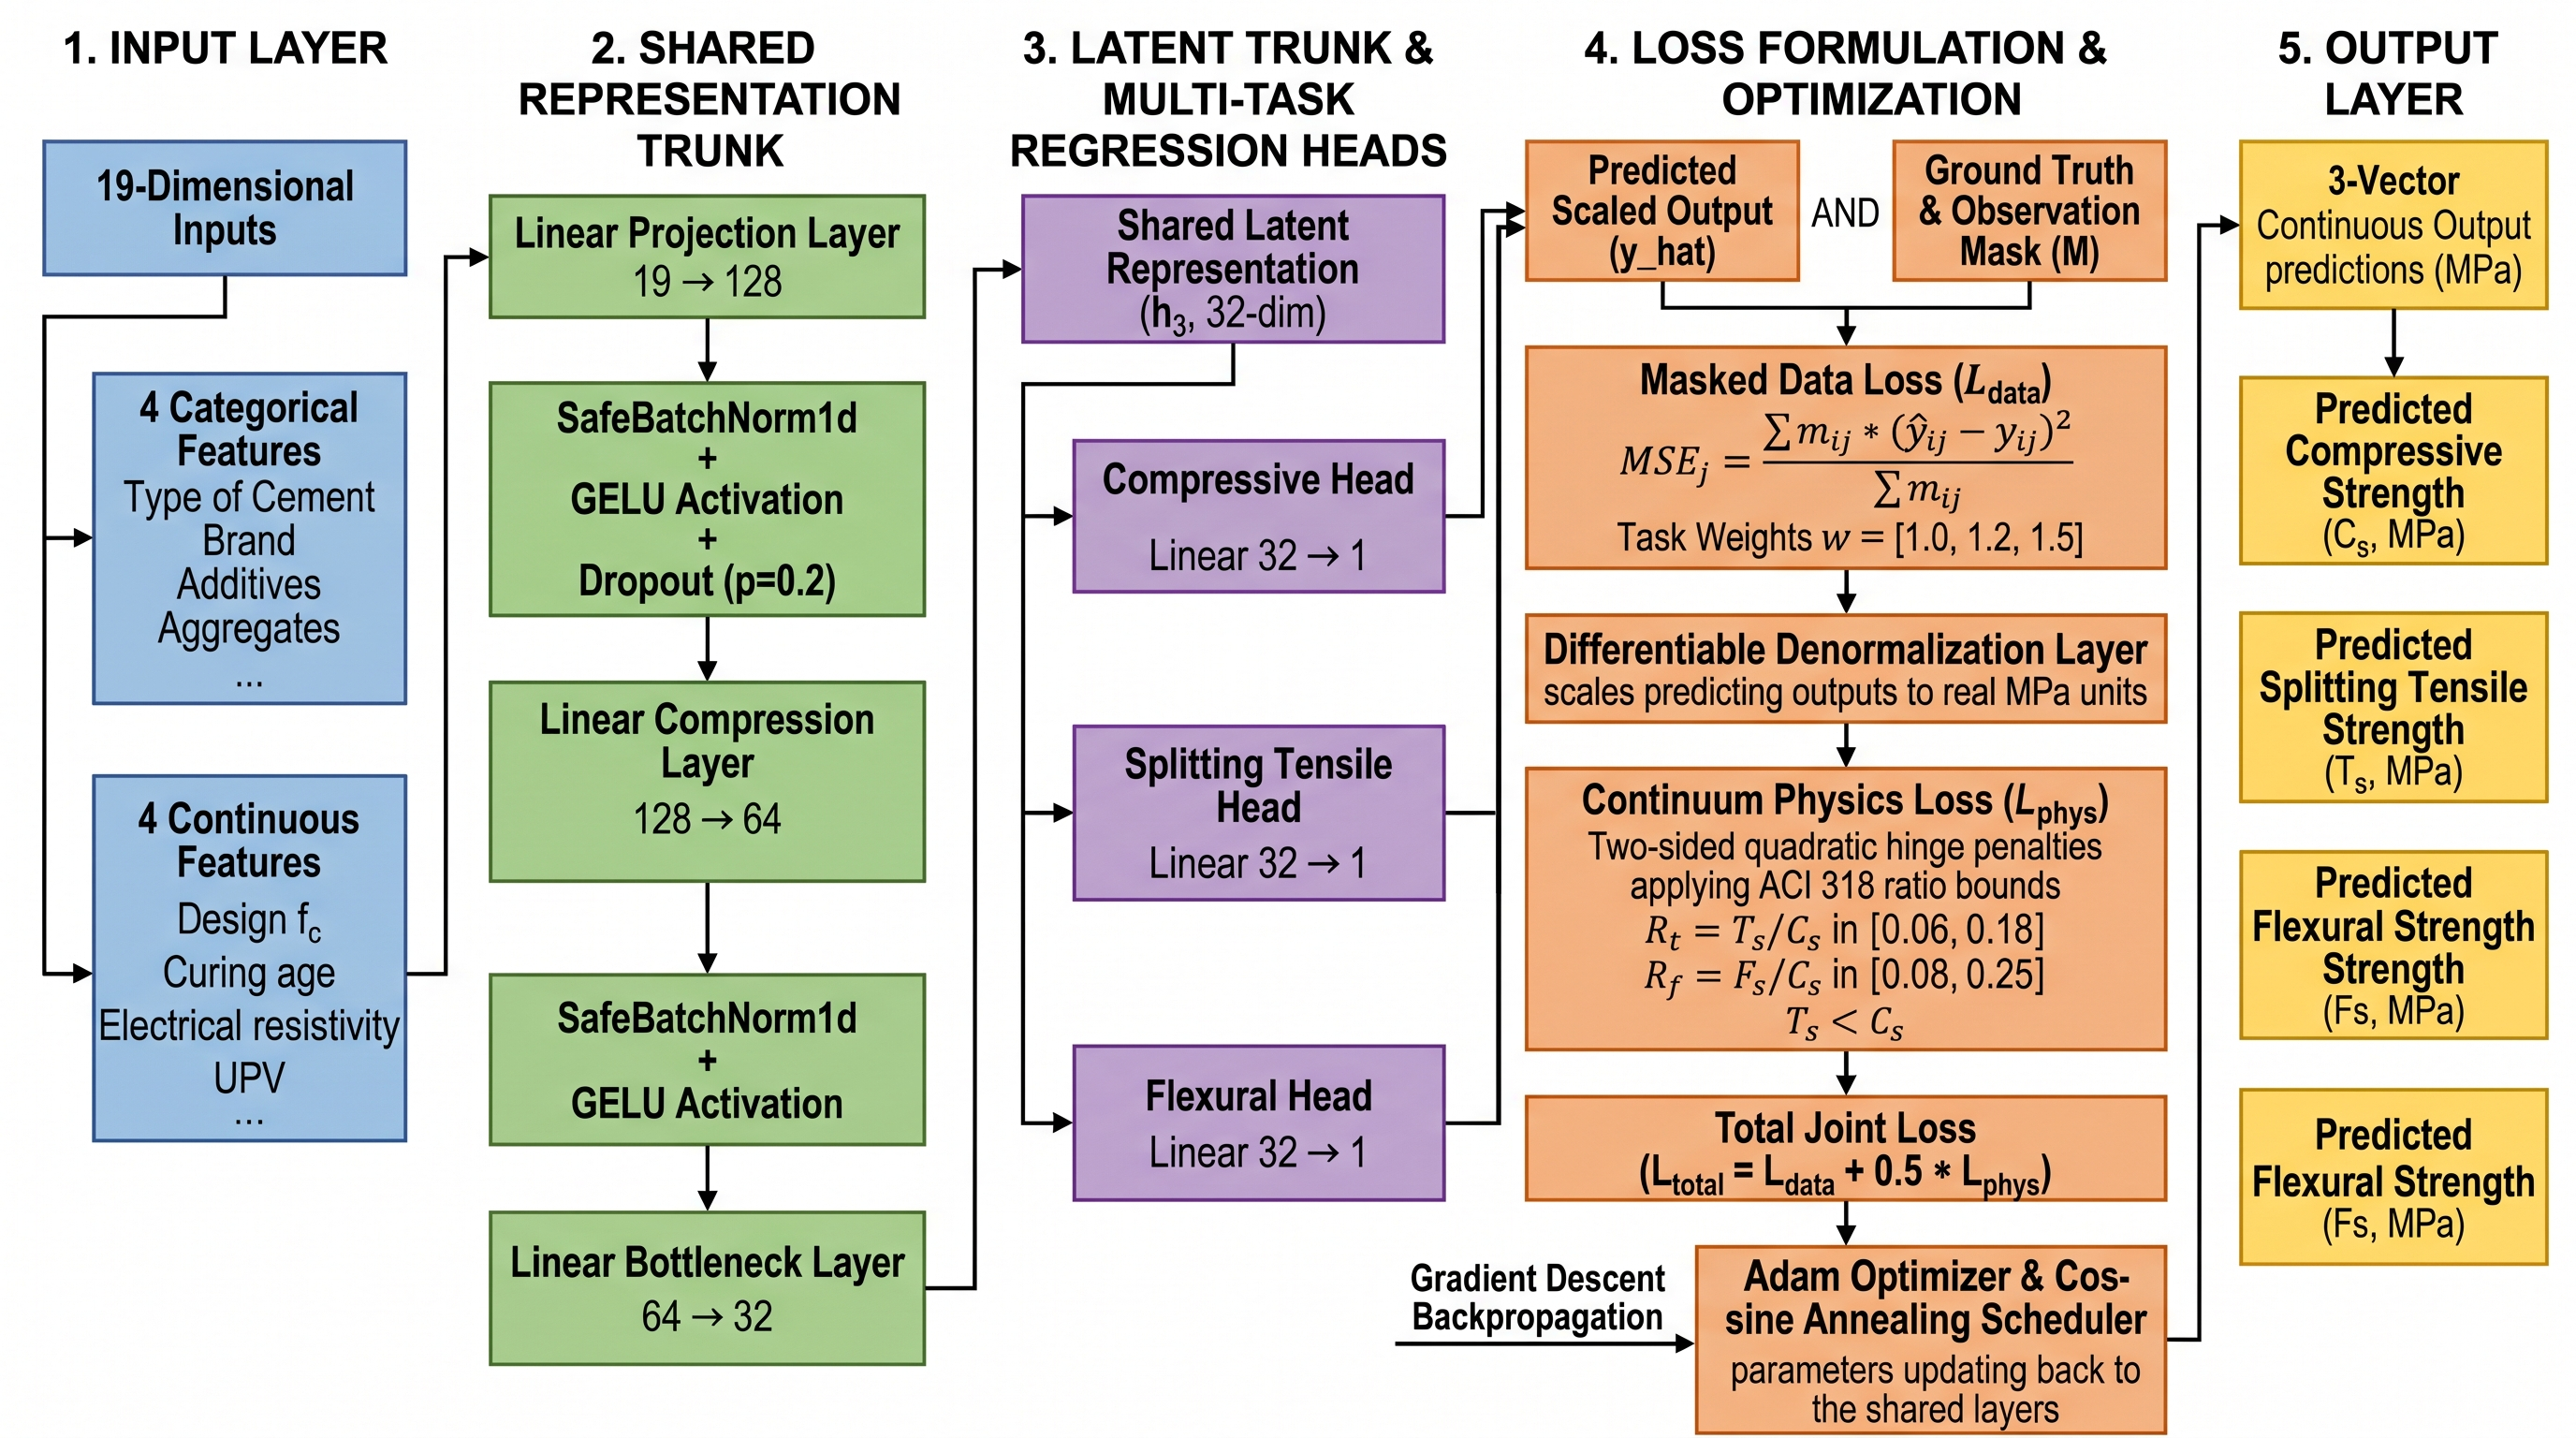
\includegraphics[width=0.96\textwidth]{architecture.png}
    \caption{Detailed architectural schematic of the PIM-MTL deep neural network and hybrid loss optimization engine: (1) 19-dimensional input fusion, (2) 3-layer shared parameter trunk with SafeBatchNorm1d, GELU activations, and Dropout, (3) specialized linear regression heads for compressive, tensile, and flexural strengths, (4) dual-channel loss combining masked MSE gradient gating with differentiable ACI 318 continuum physics regularizers, and (5) multi-property output predictions in physical MPa units.}
    \label{fig:network_architecture}
\end{figure*}

\subsection{Network Architecture: Shared Trunk and SafeBatchNorm1d}
The deep neural network architecture (illustrated in Fig.~\ref{fig:network_architecture}) employs hard parameter sharing across tasks to capture coupled hydration microstructures while maintaining dedicated regression heads for compressive, tensile, and flexural strengths:
\begin{equation}
    \mathbf{h}_1 = \text{Dropout}_{0.2}\Big(\text{GELU}\big(\text{SafeBN}(\mathbf{W}_1 \mathbf{x} + \mathbf{b}_1)\big)\Big), \quad \mathbf{W}_1 \in \mathbb{R}^{128 \times 19}
\end{equation}
\begin{equation}
    \mathbf{h}_2 = \text{GELU}\big(\text{SafeBN}(\mathbf{W}_2 \mathbf{h}_1 + \mathbf{b}_2)\big), \quad \mathbf{W}_2 \in \mathbb{R}^{64 \times 128}
\end{equation}
\begin{equation}
    \mathbf{h}_3 = \mathbf{W}_3 \mathbf{h}_2 + \mathbf{b}_3, \quad \mathbf{W}_3 \in \mathbb{R}^{32 \times 64}
\end{equation}
Across all layers, \texttt{PIM\_MTL\_Net} incorporates exactly 13,379 trainable parameters (13,280 in the shared trunk and 99 across the three prediction heads), ensuring high computational efficiency and fast convergence.

\subsubsection{SafeBatchNorm1d Formulation}
Standard PyTorch \texttt{nn.BatchNorm1d} evaluates batch variance via $\frac{1}{N-1} \sum (x_i - \mu)^2$. When deployed on-site or in quality control monitoring systems for single-mix prediction ($N=1$), standard batch normalization throws a runtime exception due to zero degrees of freedom. We implement \texttt{SafeBatchNorm1d}:
\begin{equation}
    \text{SafeBN}(x) = \begin{cases}
        \frac{x - \mu_{\text{running}}}{\sqrt{\sigma^2_{\text{running}} + \epsilon}} \odot \gamma + \beta, & \text{if } N=1 \text{ during training} \\
        \text{BatchNorm1d}(x), & \text{otherwise}
    \end{cases}
\end{equation}
This guarantees seamless inference in edge and real-time controller environments.

\subsubsection{Task-Specific Prediction Heads}
From the 32-dimensional shared latent trunk $\mathbf{h}_3$, three independent linear heads project to normalized target predictions:
\begin{equation}
    \hat{y}_{i,1} = \mathbf{w}_{cs}^T \mathbf{h}_{3,i} + b_{cs} \quad (\text{Compressive Head})
\end{equation}
\begin{equation}
    \hat{y}_{i,2} = \mathbf{w}_{ts}^T \mathbf{h}_{3,i} + b_{ts} \quad (\text{Tensile Head})
\end{equation}
\begin{equation}
    \hat{y}_{i,3} = \mathbf{w}_{fs}^T \mathbf{h}_{3,i} + b_{fs} \quad (\text{Flexural Head})
\end{equation}
Layers are initialized using Kaiming Normal initialization~\cite{he2015delving} to maintain unit gradient variance across GELU activations~\cite{hendrycks2016gelu}.

\subsection{Masked Multi-Task Empirical Loss ($\mathcal{L}_{\text{data}}$)}
To utilize all 4,420 specimens without data distortion, the empirical data loss is gated by the observation mask $\mathbf{m}_i$:
\begin{equation}
    \mathcal{L}_{\text{data}} = \sum_{j=1}^3 w_j \left[ \frac{\sum_{i=1}^N m_{ij} \left(y_{ij} - \hat{y}_{ij}\right)^2}{\max\left(1, \sum_{i=1}^N m_{ij}\right)} \right]
\end{equation}
where $\mathbf{w} = [1.0, 1.2, 1.5]$ balances dense versus sparse target representations.

\subsubsection{Mathematical Proof of Exact Gradient Gating}
Let us differentiate $\mathcal{L}_{\text{data}}$ with respect to the network prediction $\hat{y}_{ij}$ for specimen $i$ on task $j$:
\begin{align}
    \frac{\partial \mathcal{L}_{\text{data}}}{\partial \hat{y}_{ij}} &= \frac{\partial}{\partial \hat{y}_{ij}} \left( w_j \frac{\sum_{k=1}^N m_{kj} (y_{kj} - \hat{y}_{kj})^2}{\max(1, \sum_{k=1}^N m_{kj})} \right) \\
    &= \frac{-2 w_j m_{ij} (y_{ij} - \hat{y}_{ij})}{\sum_{k=1}^N m_{kj}}
\end{align}
\begin{itemize}
    \item \textbf{Case 1: Target Observed ($m_{ij} = 1.0$):}
    \begin{equation}
        \frac{\partial \mathcal{L}_{\text{data}}}{\partial \hat{y}_{ij}} = \frac{-2 w_j (y_{ij} - \hat{y}_{ij})}{N_{\text{obs}, j}} \neq 0 \quad (\text{Standard backprop})
    \end{equation}
    \item \textbf{Case 2: Target Missing ($m_{ij} = 0.0$):}
    \begin{equation}
        \frac{\partial \mathcal{L}_{\text{data}}}{\partial \hat{y}_{ij}} = \frac{-2 w_j \cdot 0 \cdot (0.0 - \hat{y}_{ij})}{N_{\text{obs}, j}} \equiv 0
    \end{equation}
\end{itemize}
The zero placeholder never corrupts parameter updates. Unobserved targets generate \textit{strictly zero empirical error gradient}. \hfill $\blacksquare$

\subsection{Differentiable Physics Regularization ($\mathcal{L}_{\text{phys}}$)}
During forward propagation, scaled predictions are differentiably mapped back into physical engineering units (MPa):
\begin{equation}
\begin{aligned}
    \hat{\mathbf{y}}_{\text{MPa}} &= \hat{\mathbf{y}}_{\text{scaled}} \odot \mathbf{s} + \boldsymbol{\mu} \\[6pt]
    \hat{C}_s &= \max(\hat{y}_{1,\text{MPa}}, 1.0), \quad 
    \hat{T}_s = \max(\hat{y}_{2,\text{MPa}}, 0.0), \\
    \hat{F}_s &= \max(\hat{y}_{3,\text{MPa}}, 0.0)
\end{aligned}
\end{equation}
The mechanical strength ratios are computed as:
\begin{equation}
    R_t = \frac{\hat{T}_s}{\hat{C}_s}, \qquad R_f = \frac{\hat{F}_s}{\hat{C}_s}
\end{equation}
The two-sided quadratic hinge regularizer penalizes deviations beyond code boundaries:
\begin{align}
    \mathcal{L}_{\text{phys}} = \frac{1}{N} \sum_{i=1}^N \Big[ & \text{ReLU}(R_{t,i} - 0.18)^2 + \text{ReLU}(0.06 - R_{t,i})^2 \nonumber \\
    + & \text{ReLU}(R_{f,i} - 0.25)^2 + \text{ReLU}(0.08 - R_{f,i})^2 \Big]
\end{align}

\subsubsection{Regularization of Unobserved Data}
Unlike $\mathcal{L}_{\text{data}}$, the physics penalty $\mathcal{L}_{\text{phys}}$ is evaluated across \textbf{all $N$ specimens} without masking. When a sample lacks flexural ground truth ($m_{i,3} = 0$):
\begin{equation}
    \frac{\partial \mathcal{L}_{\text{data}}}{\partial \hat{y}_{i,3}} = 0, \quad \text{yet} \quad \frac{\partial \mathcal{L}_{\text{phys}}}{\partial \hat{y}_{i,3}} = 2 \cdot \text{ReLU}(R_{f,i} - 0.25) \cdot \frac{s_3}{\hat{C}_{s,i}} \neq 0
\end{equation}
Consequently, the unobserved flexural head is constrained by continuum mechanics to remain proportional to compressive predictions, transferring microstructural knowledge from observed tasks. The total multi-task objective is:
\begin{equation}
    \mathcal{L}_{\text{total}} = \mathcal{L}_{\text{data}} + \lambda_{\text{phys}} \mathcal{L}_{\text{phys}}
\end{equation}
with $\lambda_{\text{phys}} = 0.5$.

\section{Experimental Setup}

\subsection{Training Protocol and Hyperparameters}
The network was trained for 60 epochs using the Adam optimizer~\cite{kingma2014adam} with an initial learning rate of $\eta_0 = 10^{-3}$, weight decay of $10^{-4}$, and mini-batch size of $N=64$. Learning rate scheduling followed a Cosine Annealing decay~\cite{loshchilov2016sgdr}:
\begin{equation}
    \eta_t = \eta_{\min} + \frac{1}{2}(\eta_0 - \eta_{\min})\left(1 + \cos\left(\frac{t}{T_{\max}}\pi\right)\right)
\end{equation}
with $T_{\max} = 60$ and $\eta_{\min} = 10^{-5}$. Gradient clipping was enforced at $\Vert \mathbf{g} \Vert_2 \le 5.0$ to stabilize optimization against early hinge transients. The random seed was fixed to 42 across Python, NumPy, and PyTorch.

\subsection{Evaluation Metrics}
Model performance was evaluated on unscaled test predictions using:
\begin{itemize}
    \item \textbf{Coefficient of Determination ($R^2$):}
    \begin{equation}
        R^2 = 1 - \frac{\sum_{i=1}^N m_{ij}(y_{ij} - \hat{y}_{ij})^2}{\sum_{i=1}^N m_{ij}(y_{ij} - \bar{y}_j)^2}
    \end{equation}
    \item \textbf{Root Mean Squared Error (RMSE):}
    \begin{equation}
        \text{RMSE} = \sqrt{\frac{\sum_{i=1}^N m_{ij}(y_{ij} - \hat{y}_{ij})^2}{\sum_{i=1}^N m_{ij}}}
    \end{equation}
    \item \textbf{Mean Absolute Error (MAE):}
    \begin{equation}
        \text{MAE} = \frac{\sum_{i=1}^N m_{ij} |y_{ij} - \hat{y}_{ij}|}{\sum_{i=1}^N m_{ij}}
    \end{equation}
    \item \textbf{Physical Violation Rates (PVR \%):}
    \begin{align}
        \text{PVR}_{\text{impossible}} &= \frac{100}{N_{\text{test}}} \sum_{i=1}^{N_{\text{test}}} \mathbb{I}(\hat{T}_{s,i} \ge \hat{C}_{s,i}) \\
        \text{PVR}_{\text{hier}} &= \frac{100}{N_{\text{test}}} \sum_{i=1}^{N_{\text{test}}} \mathbb{I}(\hat{T}_{s,i} \ge \hat{F}_{s,i}) \\
        \text{PVR}_t &= \frac{100}{N_{\text{test}}} \sum_{i=1}^{N_{\text{test}}} \mathbb{I}(R_{t,i} < 0.06 \lor R_{t,i} > 0.18) \\
        \text{PVR}_f &= \frac{100}{N_{\text{test}}} \sum_{i=1}^{N_{\text{test}}} \mathbb{I}(R_{f,i} < 0.08 \lor R_{f,i} > 0.25)
    \end{align}
    \item \textbf{Overall Physical Compliance Rate (PCR \%):}
    \begin{equation}
        \text{PCR} = \frac{100}{N_{\text{test}}} \sum_{i=1}^{N_{\text{test}}} \mathbb{I}\Big( (\hat{T}_{s,i} < \hat{C}_{s,i}) \land (\hat{T}_{s,i} < \hat{F}_{s,i}) \land (R_{t,i} \in [0.06, 0.18]) \land (R_{f,i} \in [0.08, 0.25]) \Big)
    \end{equation}
\end{itemize}

\section{Results and Comparative Analysis}

\begin{figure*}[t]
    \centering
    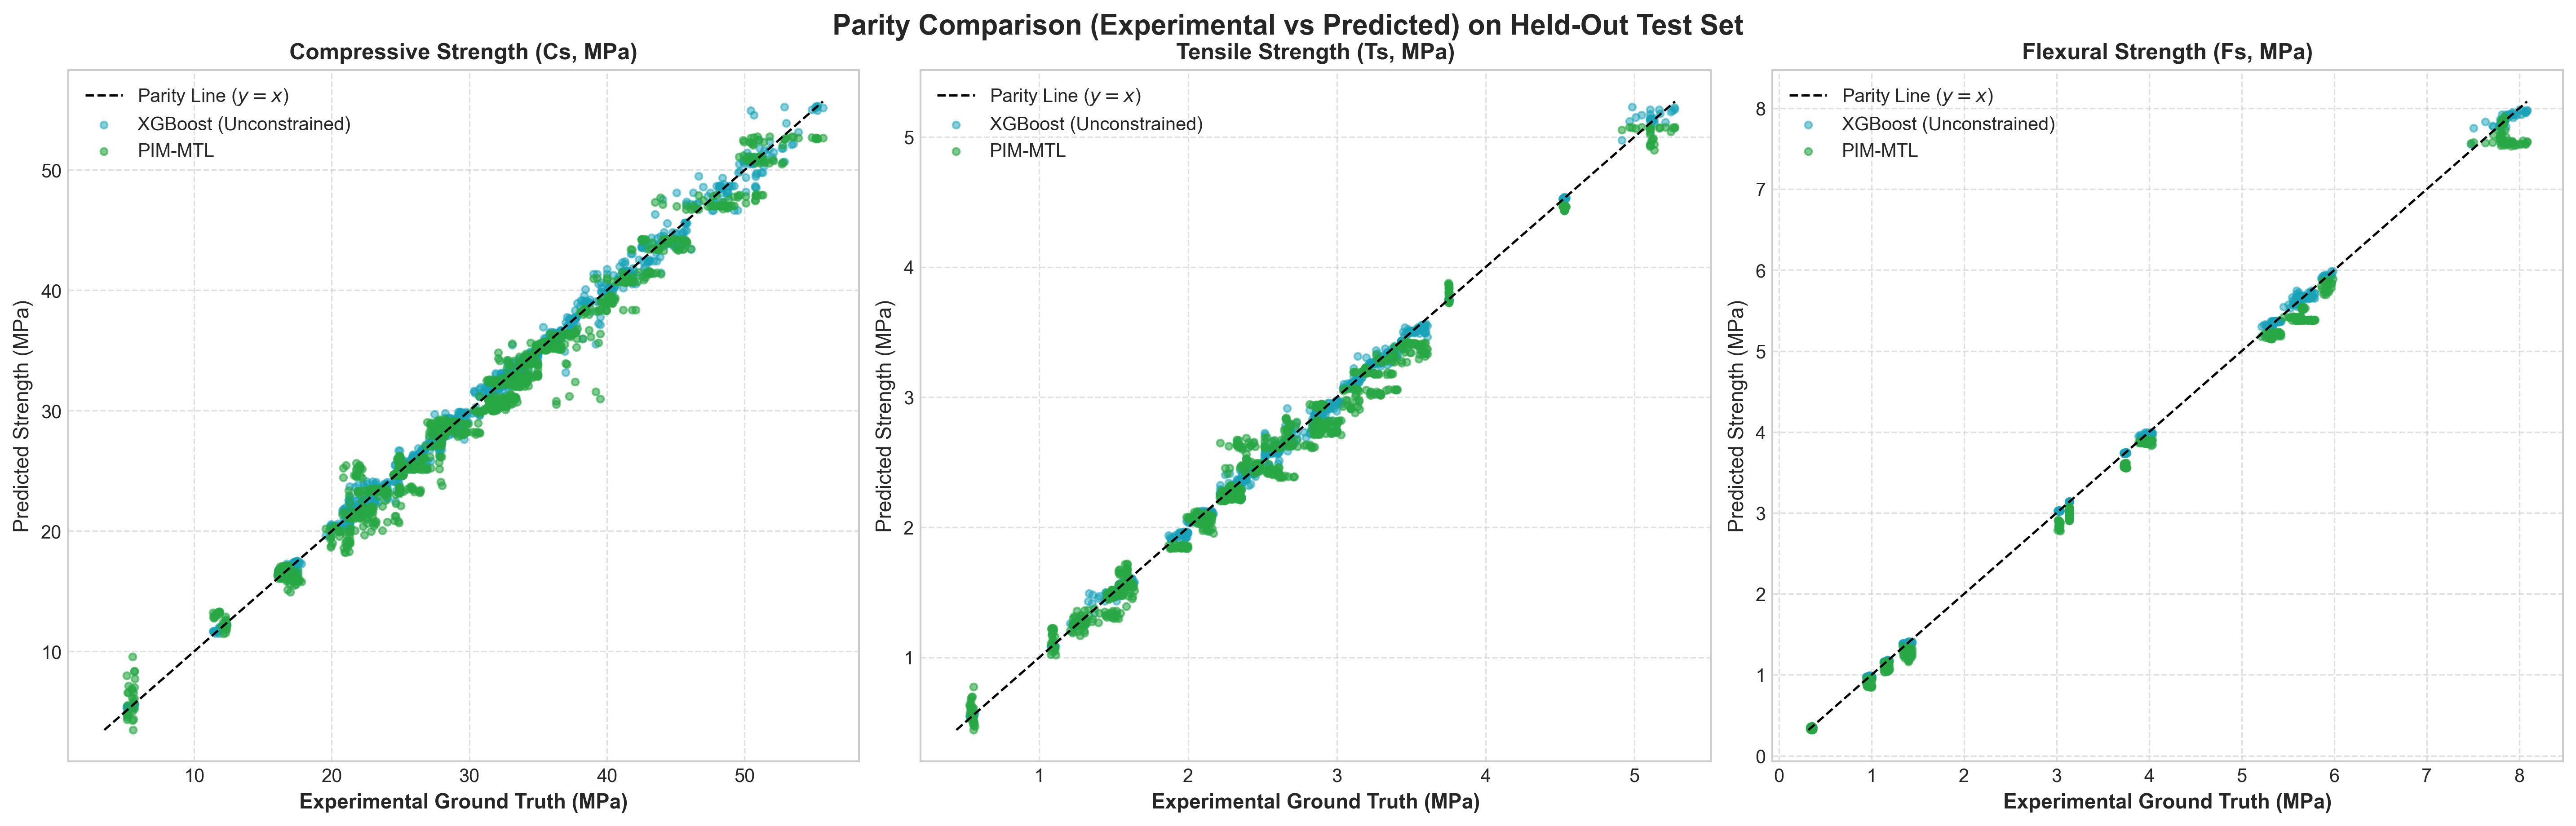
\includegraphics[width=0.98\textwidth]{actual_vs_predicted_parity.png}
    \caption{Parity plots ($y = x$) comparing experimental laboratory ground truth versus model predictions on the held-out 30\% test split ($N_{\text{test}}=1,326$) across Compressive Strength ($C_s$), Splitting Tensile Strength ($T_s$), and Flexural Strength ($F_s$). Predictions from unconstrained XGBoost regression (cyan) are contrasted with the proposed PIM-MTL framework (green) against the ideal parity line (dashed black).}
    \label{fig:parity_plots}
\end{figure*}

\begin{figure*}[t]
    \centering
    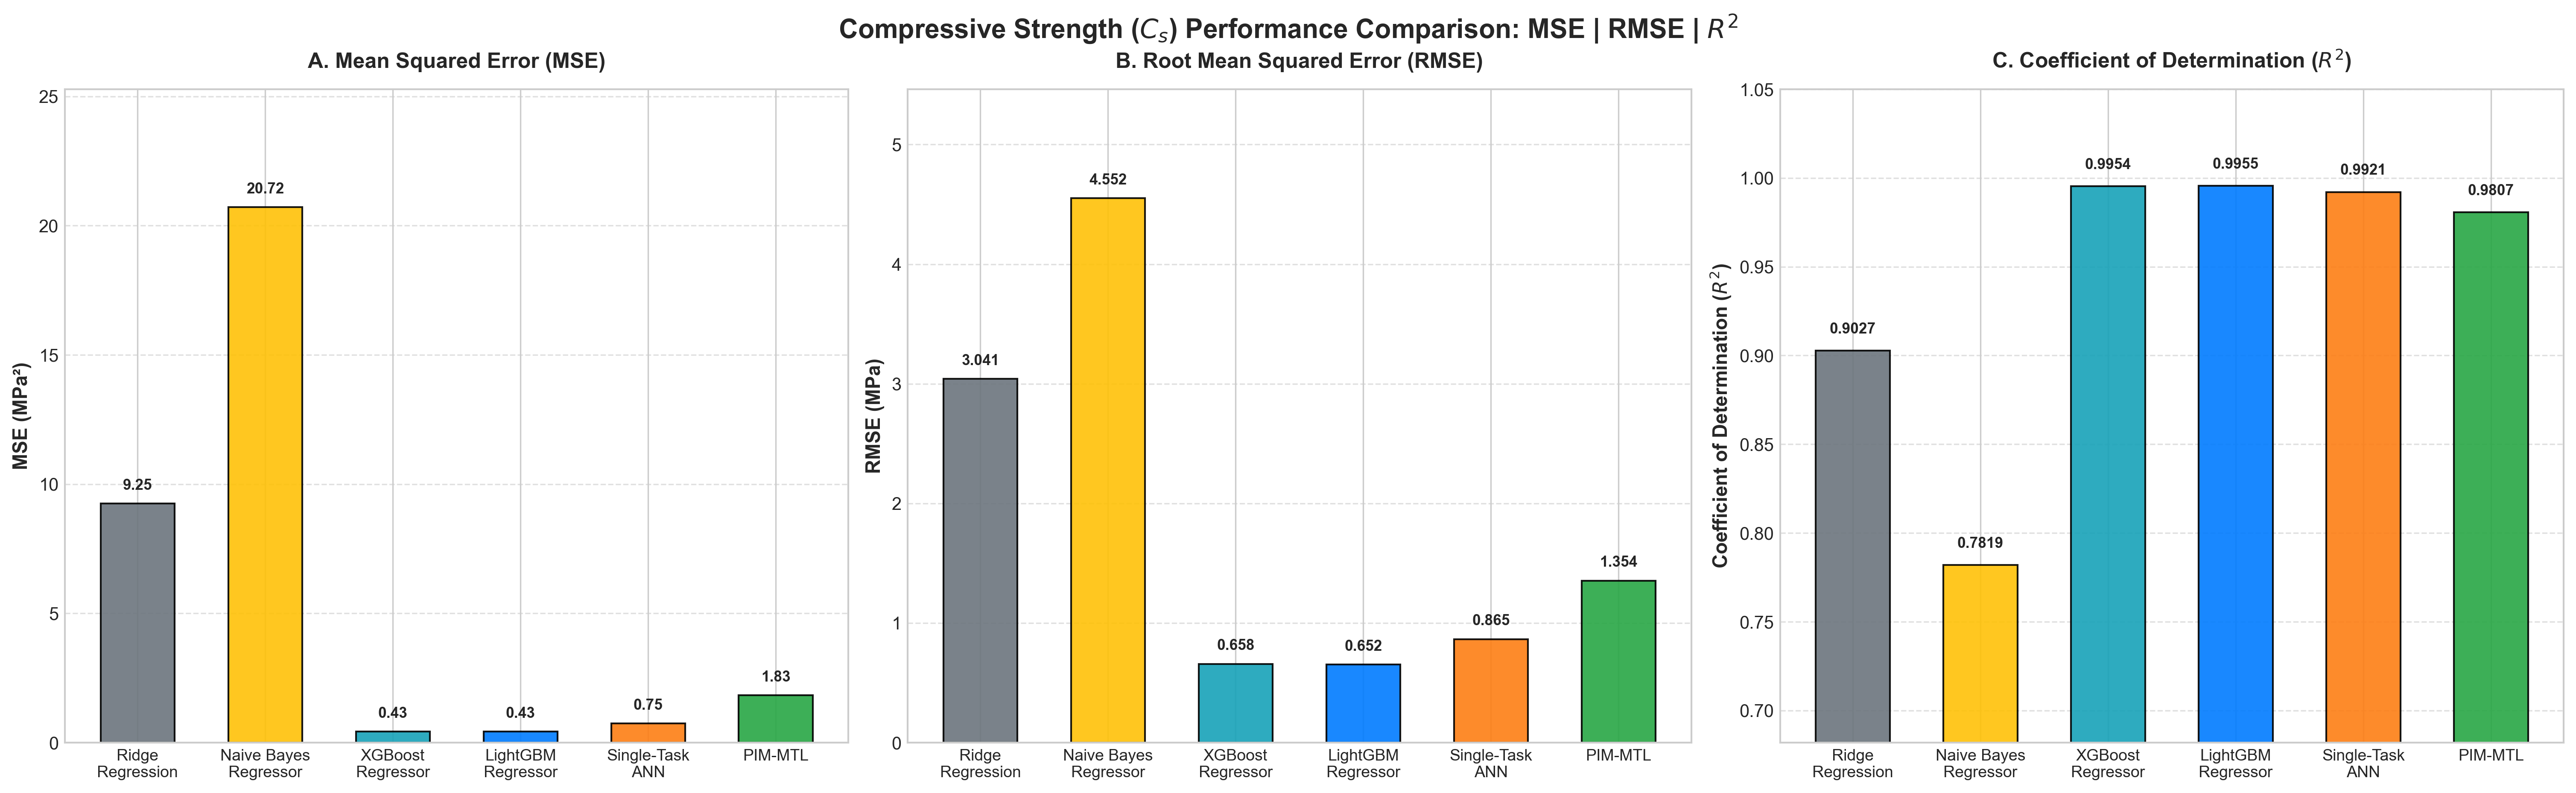
\includegraphics[width=0.98\textwidth]{cs_performance_comparison.png}
    \caption{Compressive Strength ($C_s$, MPa) benchmark across all candidate models on the 30\% held-out test split: (A) Mean Squared Error (MSE), (B) Root Mean Squared Error (RMSE), and (C) Coefficient of Determination ($R^2$). Model names are wrapped to prevent overlap.}
    \label{fig:cs_metrics}
\end{figure*}

\begin{figure*}[t]
    \centering
    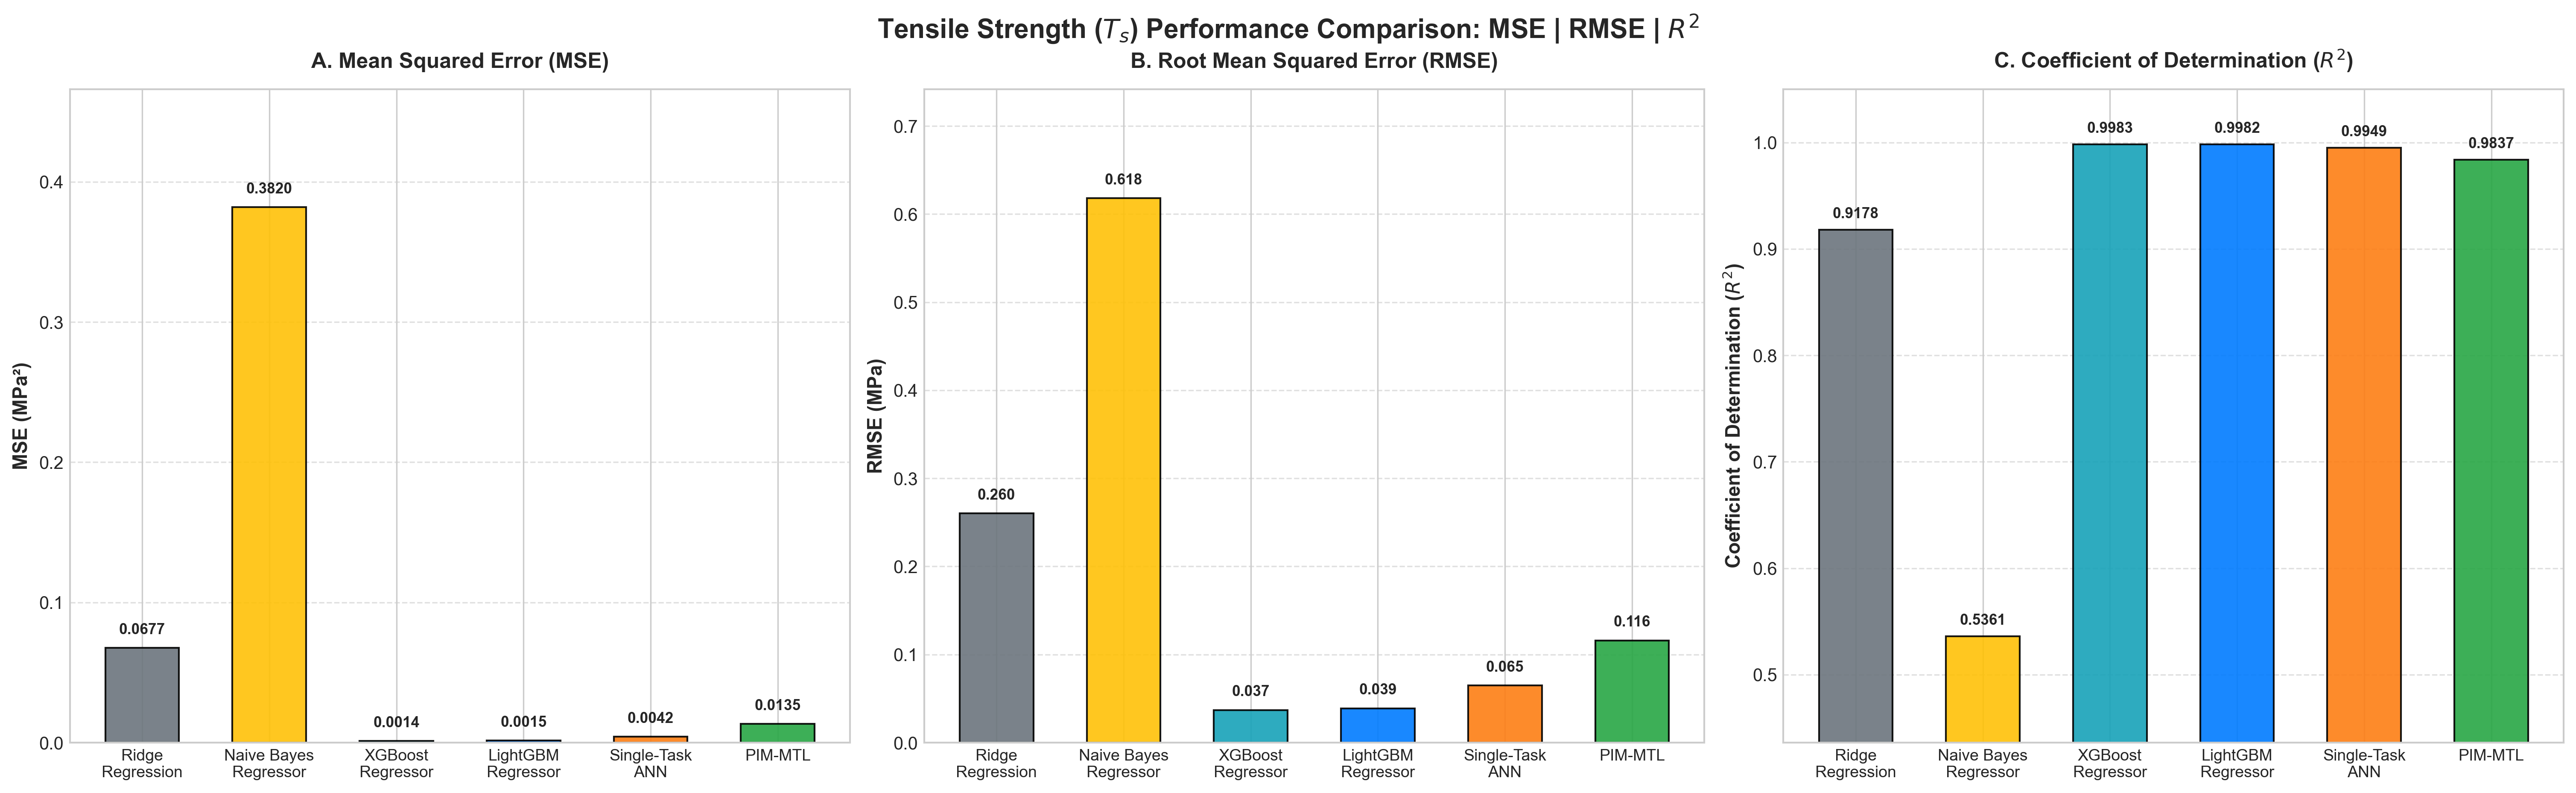
\includegraphics[width=0.98\textwidth]{ts_performance_comparison.png}
    \caption{Splitting Tensile Strength ($T_s$, MPa) benchmark across candidate models: (A) Mean Squared Error (MSE), (B) Root Mean Squared Error (RMSE), and (C) Coefficient of Determination ($R^2$) across $N=1,041$ observed test specimens.}
    \label{fig:ts_metrics}
\end{figure*}

\begin{figure*}[t]
    \centering
    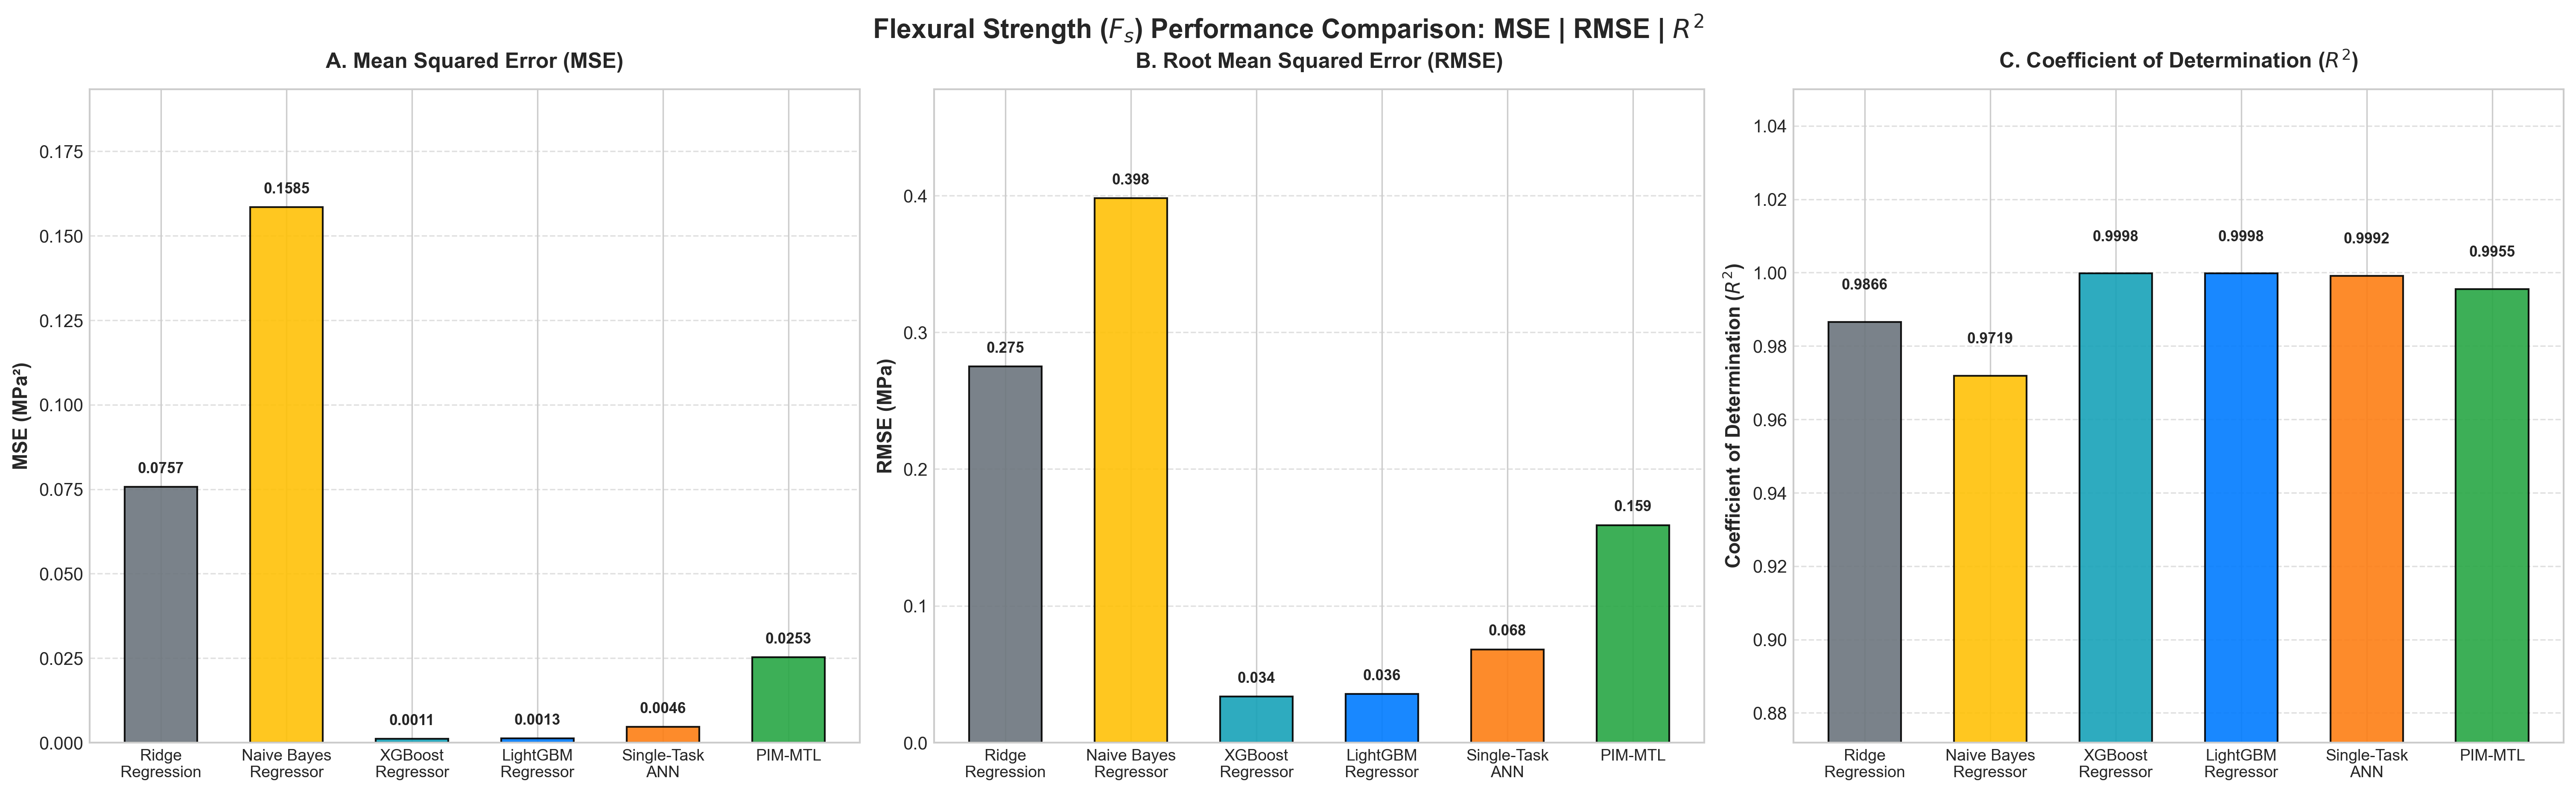
\includegraphics[width=0.98\textwidth]{fs_performance_comparison.png}
    \caption{Flexural Strength ($F_s$, MPa) benchmark across candidate models: (A) Mean Squared Error (MSE), (B) Root Mean Squared Error (RMSE), and (C) Coefficient of Determination ($R^2$). Despite $F_s$ being observed in only 40.9\% of test mixes ($N=542$), PIM-MTL achieves $R^2 = 0.9955$ and $\text{RMSE} = 0.1590$~MPa via multi-task representation transfer.}
    \label{fig:fs_metrics}
\end{figure*}

\begin{figure*}[t]
    \centering
    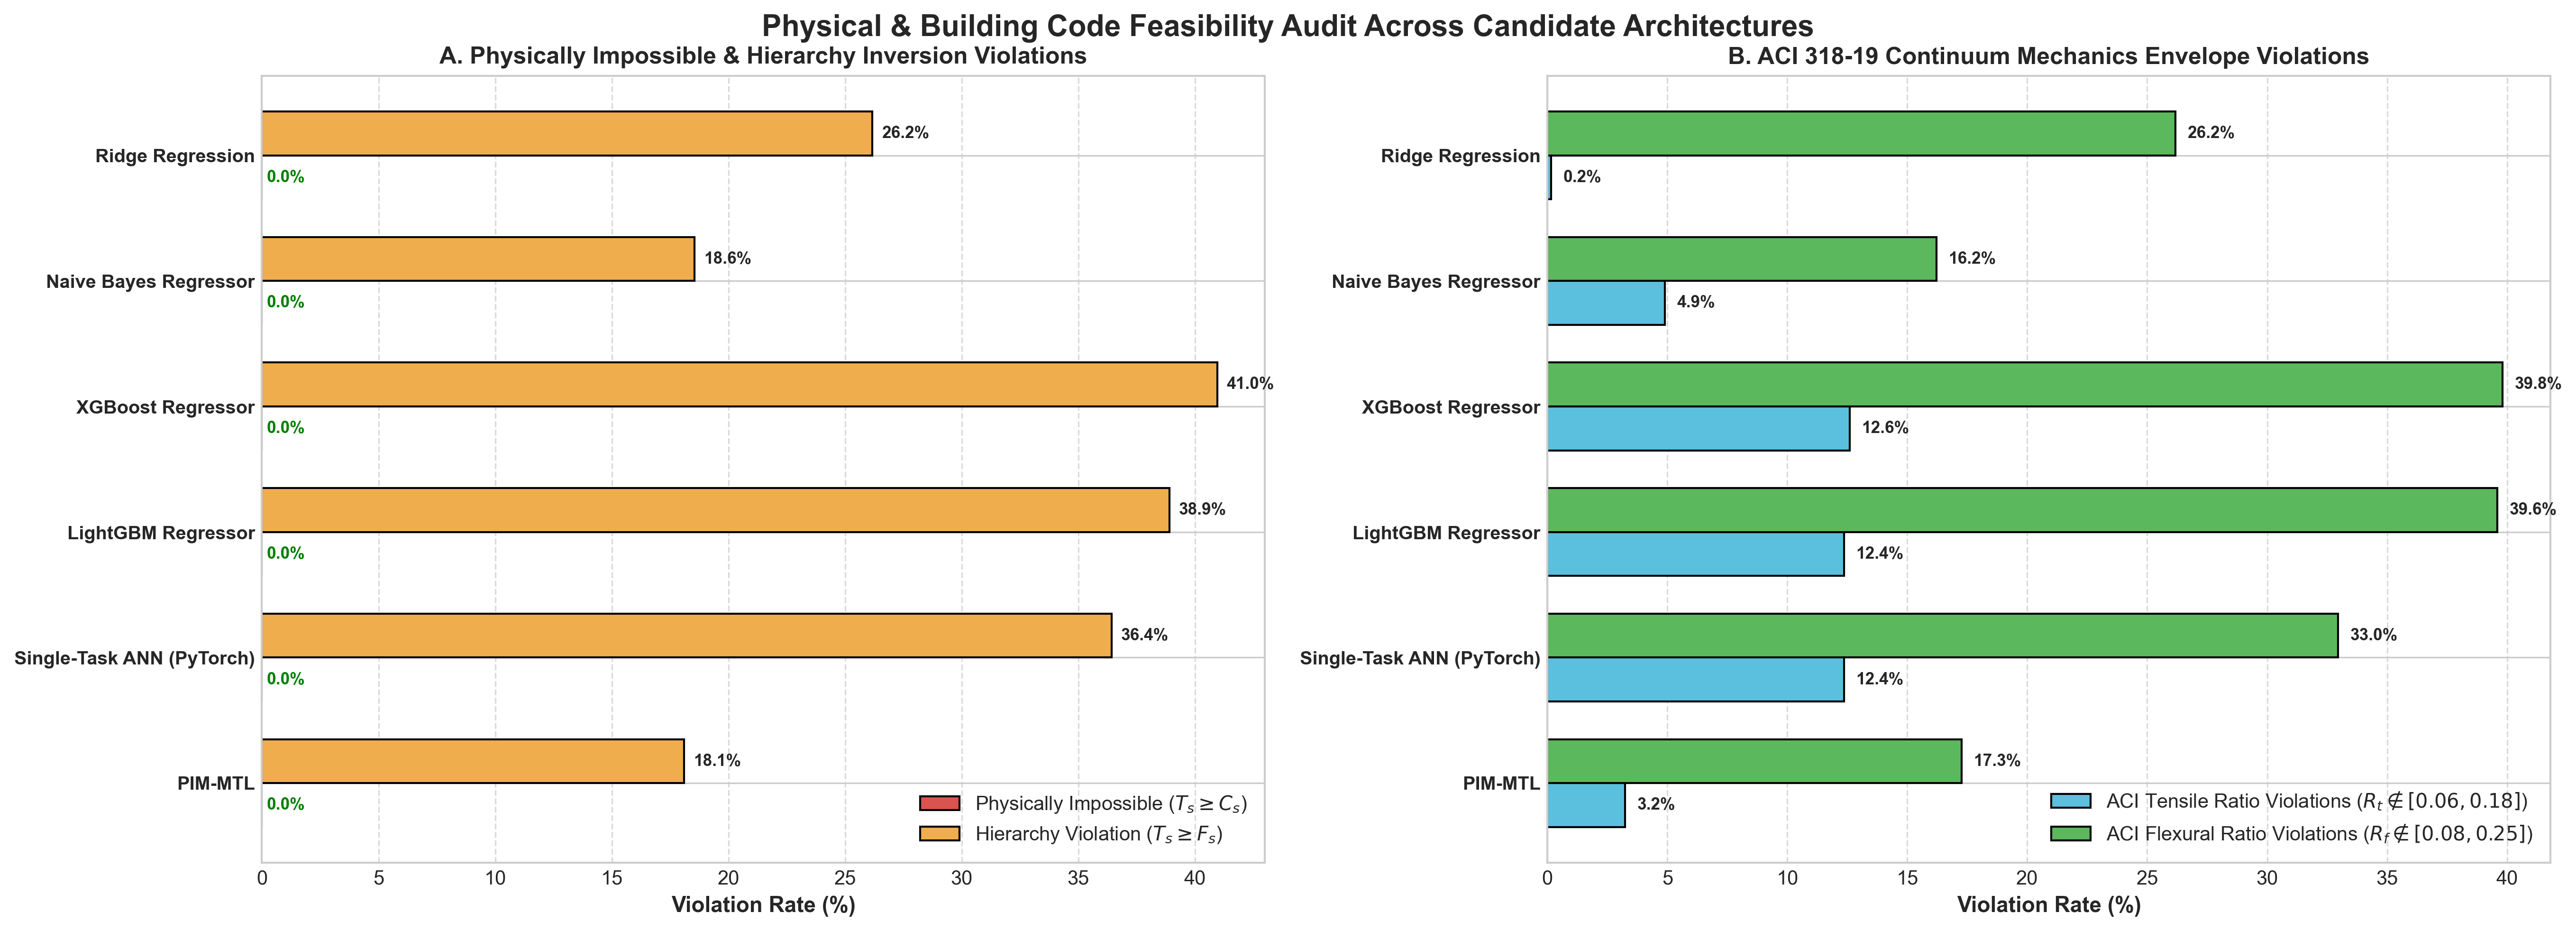
\includegraphics[width=0.95\textwidth]{physical_violation_rates.png}
    \caption{Physical and building code feasibility audit across candidate architectures on the 30\% held-out test split ($N_{\text{test}}=1,326$): (A) Severe inversion violations, contrasting physically impossible predictions ($T_s \ge C_s$) and strength hierarchy inversions ($T_s \ge F_s$); (B) ACI 318-19 continuum mechanics ratio violations for tensile ($R_t \notin [0.06, 0.18]$) and flexural ($R_f \notin [0.08, 0.25]$) envelopes.}
    \label{fig:physical_violations}
\end{figure*}

\begin{figure*}[t]
    \centering
    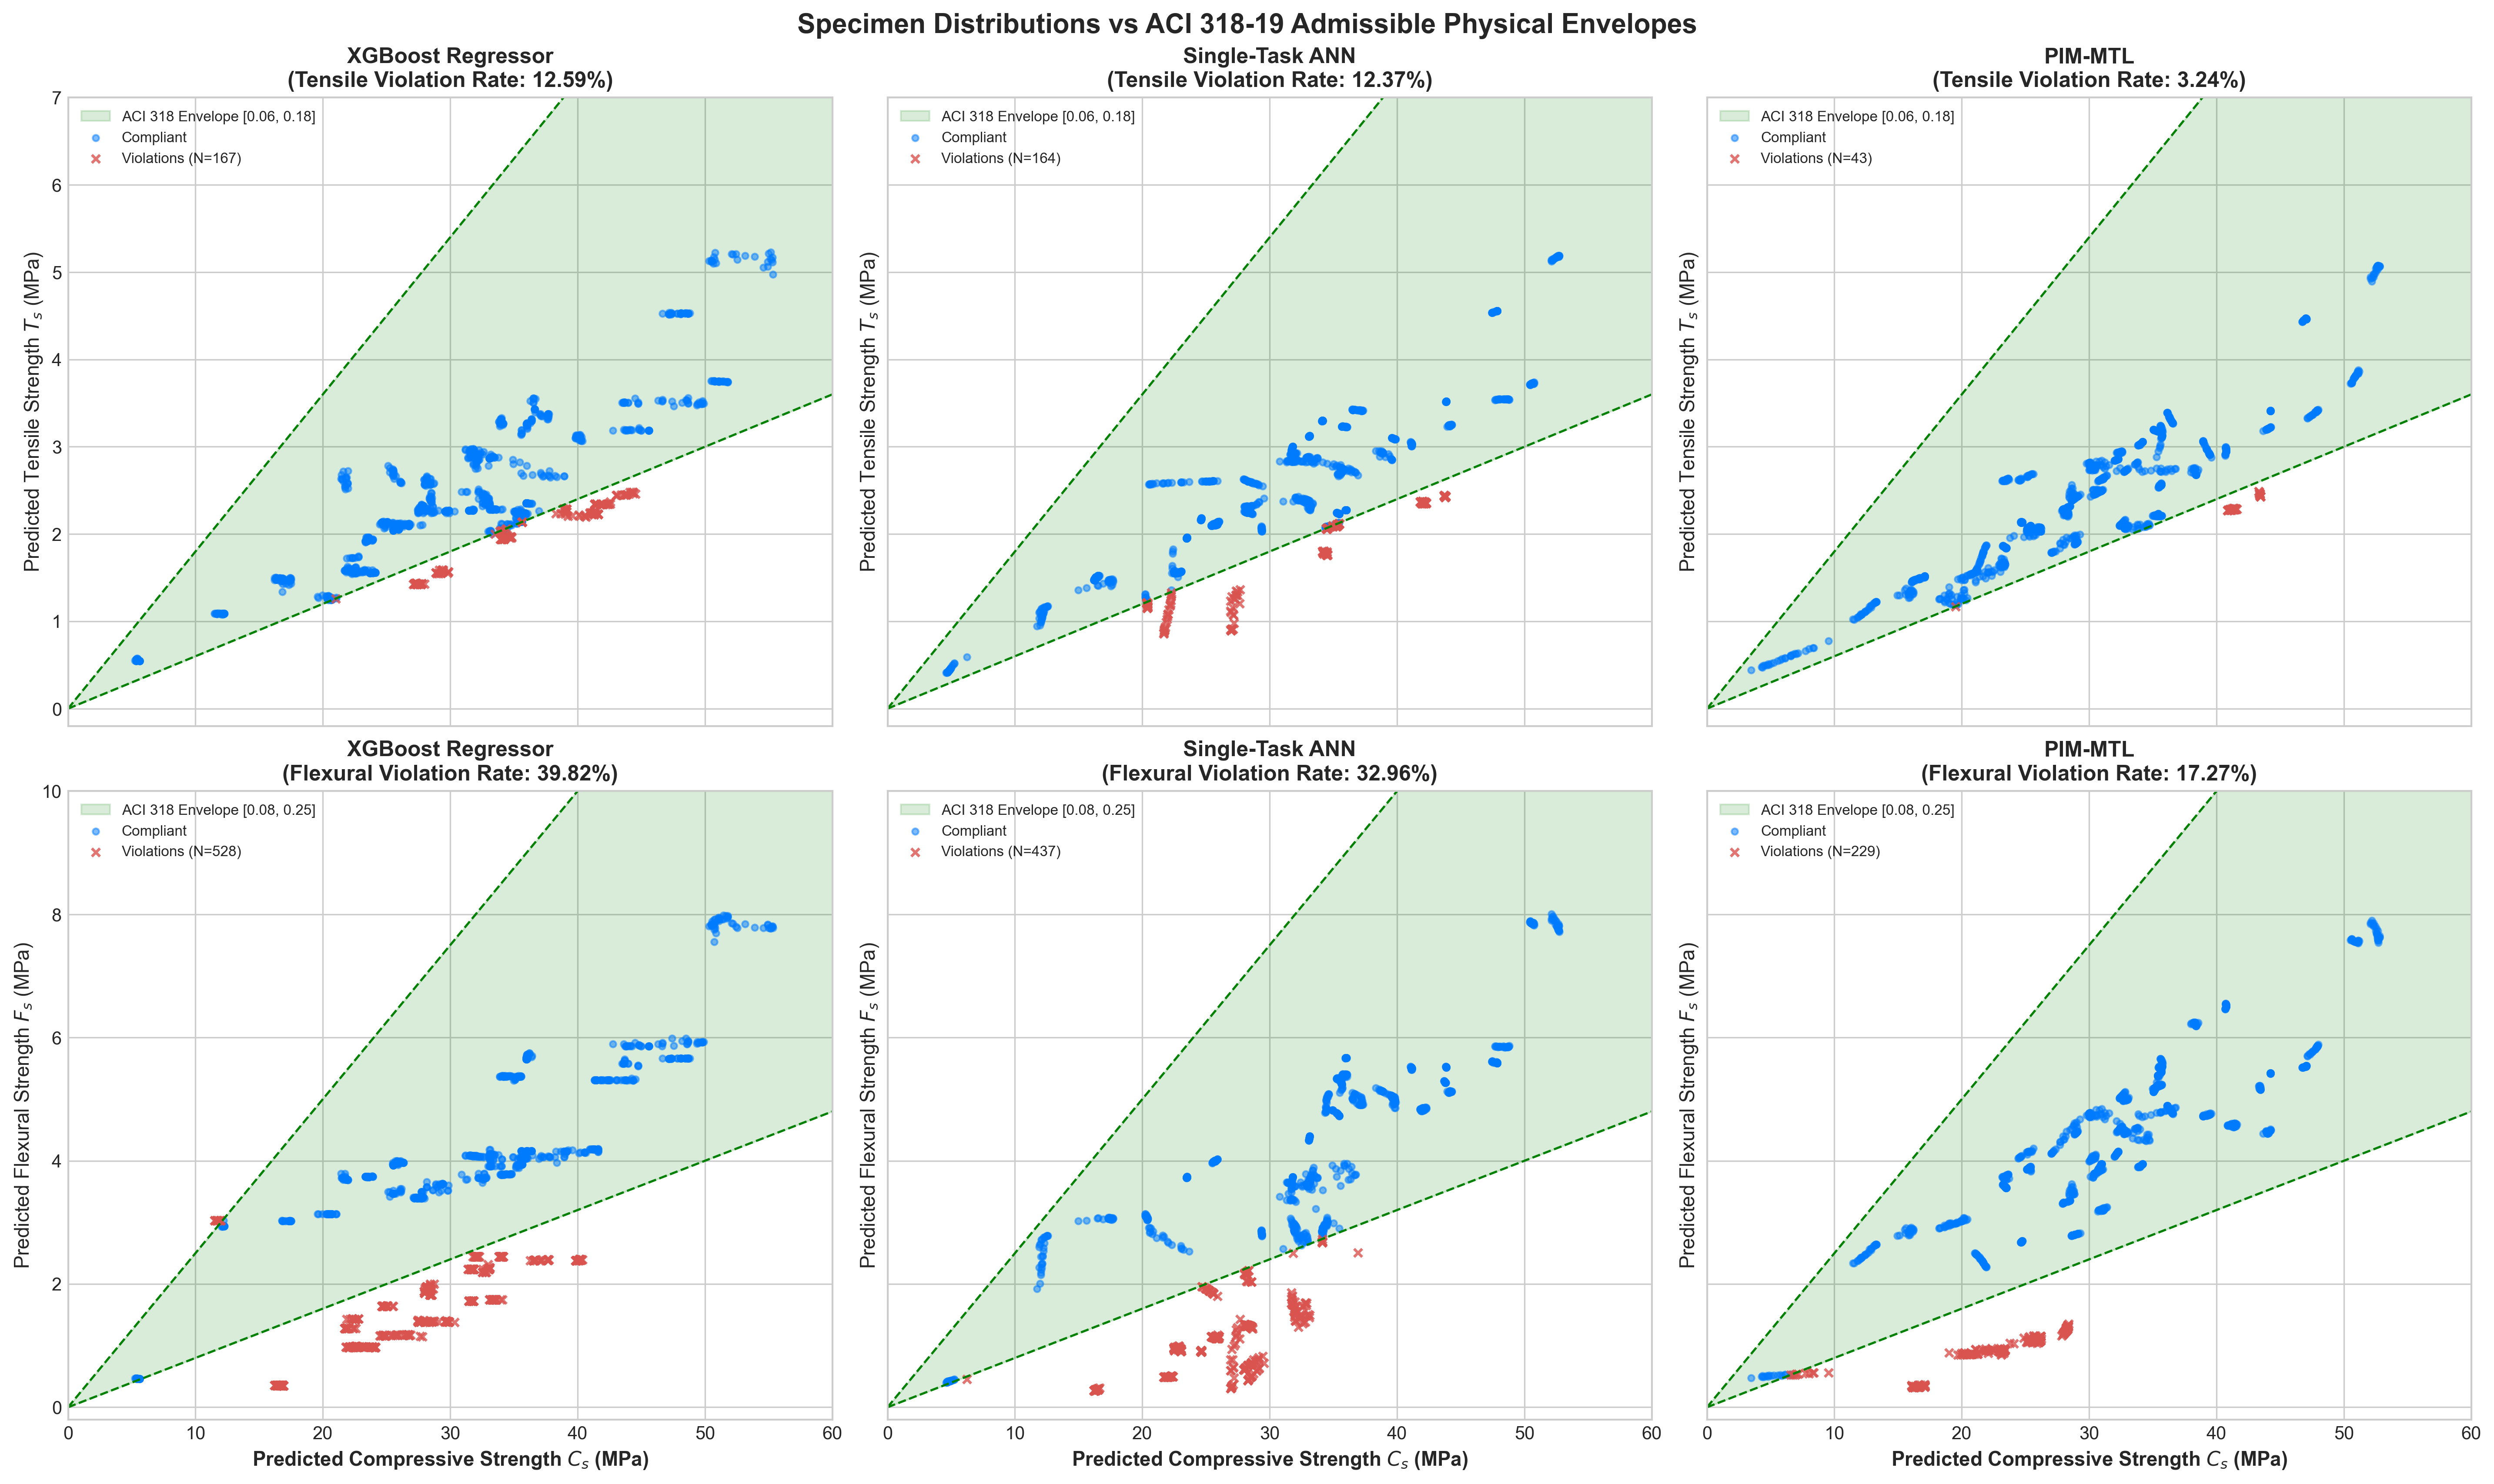
\includegraphics[width=0.98\textwidth]{aci_constraint_envelopes.png}
    \caption{Specimen predictions plotted against shaded ACI 318-19 admissible physical envelopes ($0.06 \le R_t \le 0.18$ and $0.08 \le R_f \le 0.25$) across the test set for unconstrained XGBoost, Single-Task ANN, and PIM-MTL. Blue dots indicate code-compliant specimens; red cross markers designate code-violating outliers, demonstrating severe structural violations by unconstrained models.}
    \label{fig:aci_envelopes}
\end{figure*}

\begin{figure*}[t]
    \centering
    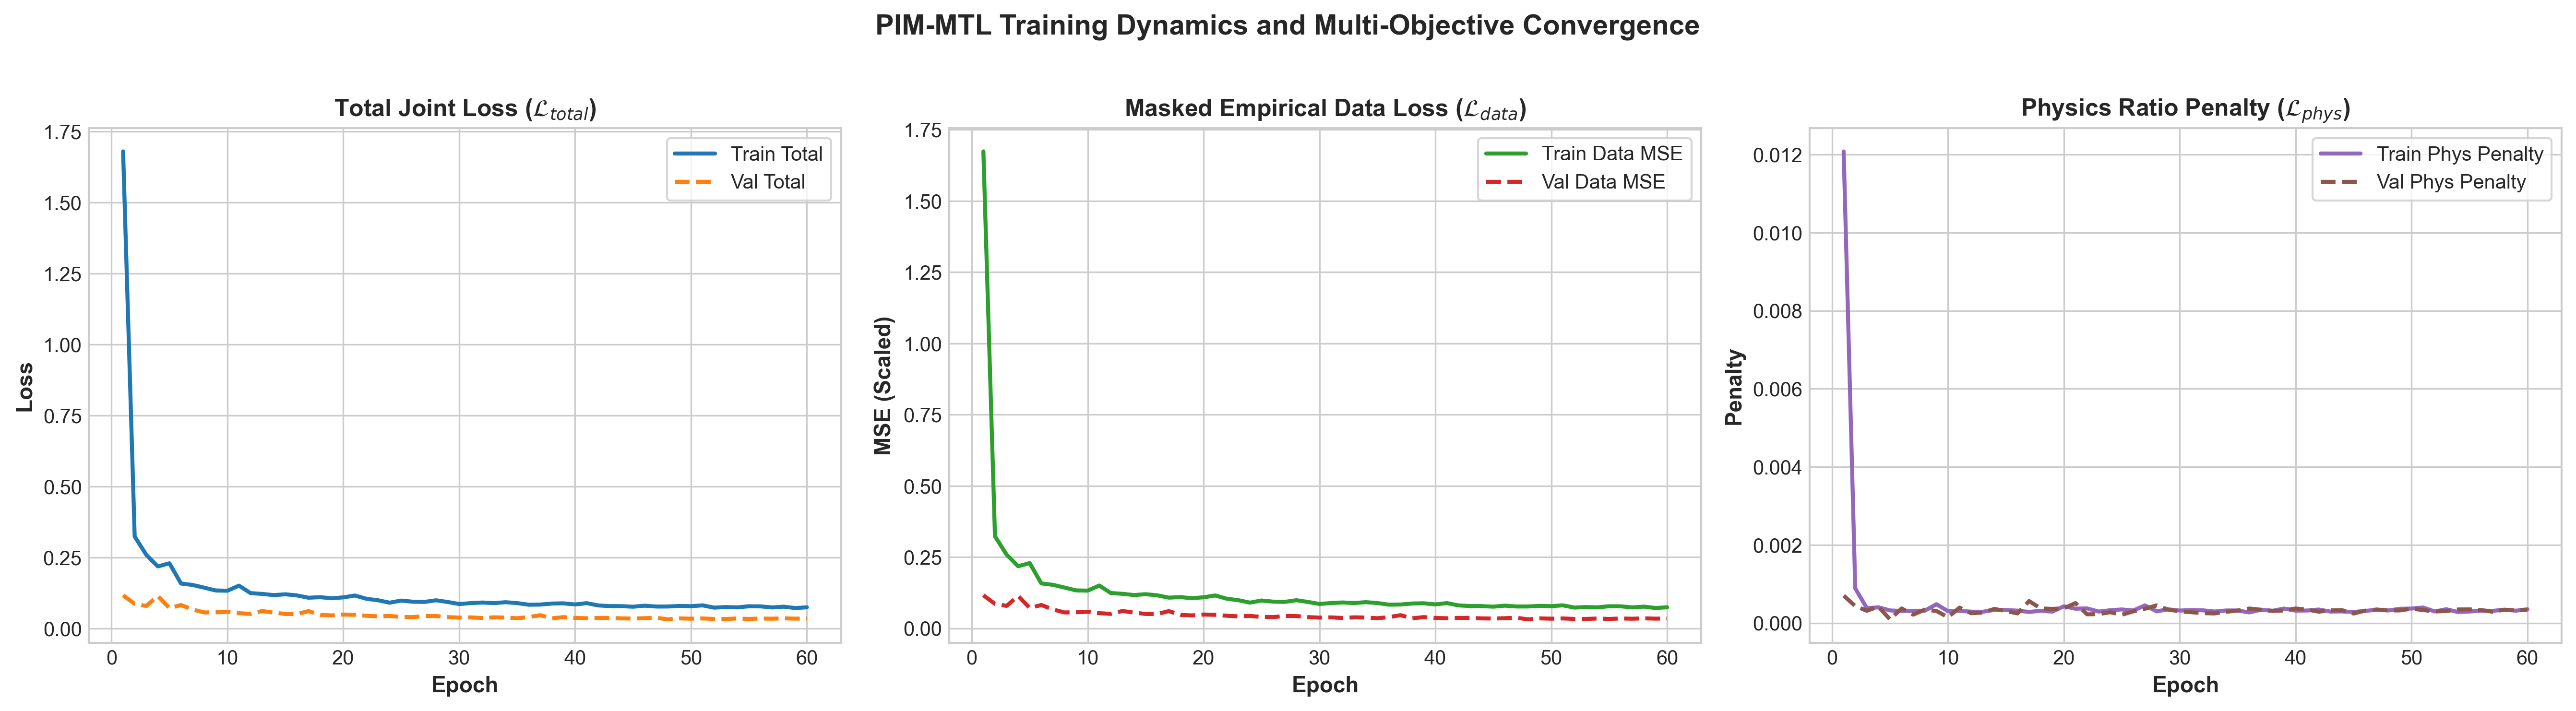
\includegraphics[width=0.92\textwidth]{08_training_convergence_curves.png}
    \caption{Training loss convergence across 60 epochs: Total Loss (left), Masked Data MSE (center), and Physics Penalty (right).}
    \label{fig:convergence}
\end{figure*}

\subsection{Training Convergence Dynamics}
Fig.~\ref{fig:convergence} tracks the training loss trajectories over 60 epochs. In the initial epoch, the physics penalty starts at $0.012079$. Within the first 10 epochs, the physics loss drops by \textbf{97.7\%} to $0.000279$, confirming that the parameter-shared latent trunk rapidly maps representations into code-compliant ratio envelopes before fine-tuning empirical precision. By epoch 60, total loss smoothly converges to $0.0745$ (Data MSE: $0.0744$, Physics penalty: $0.000315$).

\subsection{Quantitative Test Set Performance}
Table~\ref{tab:results_summary} presents the target-specific performance metrics of PIM-MTL on the standardized 30\% held-out test partition ($N_{\text{test}} = 1,326$, seed 42). Compressive strength achieves $R^2 = 0.9807$ ($\text{Adj. } R^2 = 0.9806$, $\text{RMSE} = 1.3538$~MPa, $\text{MAE} = 1.0199$~MPa), representing an average relative error of only 3.27\% on a 31.2~MPa baseline across all 1,326 test mixes. Splitting tensile strength achieves $R^2 = 0.9837$ ($\text{Adj. } R^2 = 0.9835$, $\text{RMSE} = 0.1160$~MPa, $\text{MAE} = 0.0895$~MPa) across 1,041 observed specimens. 

Most notably, flexural strength achieves $R^2 = 0.9955$ ($\text{Adj. } R^2 = 0.9954$, $\text{RMSE} = 0.1590$~MPa, $\text{MAE} = 0.1296$~MPa) across the 542 observed test specimens. Despite being unobserved in 59.1\% of test mixes, the flexural head achieves sub-0.16~MPa root mean squared error, verifying that masked multi-task gradient gating successfully transfers hydration and maturity features learned from the complete compressive target to sparse flexural rupture prediction without requiring synthetic imputation.

\begin{table}[t]
\caption{Quantitative Test Set Evaluation Metrics for PIM-MTL ($N_{\text{test}} = 1,326$, 30\% Split)}
\label{tab:results_summary}
\centering
\footnotesize
\setlength{\tabcolsep}{3.5pt}
\renewcommand{\arraystretch}{1.15}
\begin{tabularx}{\columnwidth}{@{}>{\raggedright\arraybackslash}Xcccccc@{}}
\toprule
\textbf{Target} & \textbf{Obs.} & \textbf{Coverage} & \textbf{$R^2$} & \textbf{Adj. $R^2$} & \textbf{RMSE} & \textbf{MAE} \\
\midrule
Compressive ($C_s$) & 1,326 & 100.0\% & 0.9807 & 0.9806 & 1.3538 & 1.0199 \\
Tensile ($T_s$)     & 1,041 & 78.5\%  & 0.9837 & 0.9835 & 0.1160 & 0.0895 \\
Flexural ($F_s$)    & 542   & 40.9\%  & 0.9955 & 0.9954 & 0.1590 & 0.1296 \\
\bottomrule
\end{tabularx}
\vspace{0.3ex}
\parbox{\columnwidth}{\footnotesize RMSE and MAE values are reported in MPa. Fixed test split generated with seed 42.}
\end{table}

\begin{table*}[t]
\caption{Comprehensive Benchmark Comparison and ACI 318 Physical Compliance Audit on 30\% Held-Out Test Set ($N_{\text{test}} = 1,326$)}
\label{tab:baseline_comparison}
\centering
\scriptsize
\setlength{\tabcolsep}{3pt}
\renewcommand{\arraystretch}{1.20}
\begin{tabular*}{\textwidth}{@{\extracolsep{\fill}} l c c c c c c c c c c c @{}}
\toprule
\multirow{2}{*}{\textbf{Model Architecture}} & \multicolumn{2}{c}{\textbf{Compressive ($C_s$)}} & \multicolumn{2}{c}{\textbf{Tensile ($T_s$)}} & \multicolumn{2}{c}{\textbf{Flexural ($F_s$)}} & \multicolumn{4}{c}{\textbf{Physical Constraint Violation Rates (\%)}} & \multirow{2}{*}{\textbf{Overall Compliance}} \\
\cmidrule(lr){2-3} \cmidrule(lr){4-5} \cmidrule(lr){6-7} \cmidrule(lr){8-11}
& $R^2$ & RMSE & $R^2$ & RMSE & $R^2$ & RMSE & $T_s \ge C_s$ & $T_s \ge F_s$ & ACI $R_t$ & ACI $R_f$ & \\
\midrule
Ridge Regression           & 0.9027 & 3.0408 & 0.9178 & 0.2601 & 0.9866 & 0.2751 & \textbf{0.00\%} & 26.17\% & \textbf{0.15\%} & 26.17\% & 73.68\% \\
Naive Bayes Regressor      & 0.7819 & 4.5520 & 0.5361 & 0.6181 & 0.9719 & 0.3981 & \textbf{0.00\%} & 18.55\% & 4.90\%          & 16.21\% & 72.47\% \\
XGBoost Regressor          & 0.9954 & 0.6579 & 0.9983 & 0.0370 & 0.9998 & 0.0337 & \textbf{0.00\%} & 40.95\% & 12.59\%         & 39.82\% & 45.55\% \\
LightGBM Regressor         & 0.9955 & 0.6520 & 0.9982 & 0.0388 & 0.9998 & 0.0355 & \textbf{0.00\%} & 38.91\% & 12.37\%         & 39.59\% & 48.04\% \\
Single-Task ANN (PyTorch)  & 0.9921 & 0.8652 & 0.9949 & 0.0648 & 0.9992 & 0.0682 & \textbf{0.00\%} & 36.43\% & 12.37\%         & 32.96\% & 54.60\% \\
\midrule
\textbf{PIM-MTL (Proposed)} & \textbf{0.9807} & \textbf{1.3538} & \textbf{0.9837} & \textbf{0.1160} & \textbf{0.9955} & \textbf{0.1590} & \textbf{0.00\%} & \textbf{18.10\%} & \textbf{3.24\%} & \textbf{17.27\%} & \textbf{78.66\%} \\
\bottomrule
\end{tabular*}
\vspace{0.4ex}
\parbox{\textwidth}{\footnotesize RMSE values are reported in MPa. $T_s \ge C_s$ denotes physically impossible predictions (direct tensile exceeding compressive capacity). $T_s \ge F_s$ denotes structural hierarchy inversion violations. ACI $R_t$ and $R_f$ denote violations of the ACI 318-19 envelopes ($0.06 \le R_t \le 0.18$ and $0.08 \le R_f \le 0.25$). Overall Compliance denotes the percentage of specimens that satisfy all four physical invariants simultaneously.}
\end{table*}

\subsection{Cross-Architecture Benchmark and The Metric Illusion}
Table~\ref{tab:baseline_comparison} and Figs.~\ref{fig:cs_metrics}, \ref{fig:ts_metrics}, and \ref{fig:fs_metrics} compare PIM-MTL against five supervised baseline models: Ridge Regression, Naive Bayes Regressor (20 quantile bins), XGBoost Regressor, LightGBM Regressor, and a dedicated Single-Task PyTorch ANN.

At first glance, gradient boosted decision trees (XGBoost and LightGBM) appear to attain near-flawless empirical metrics ($R^2 > 0.995$ on $C_s$, and $R^2 > 0.998$ on $T_s$ and $F_s$), while the Single-Task ANN reaches $R^2 > 0.992$. However, when audited for civil engineering validity, these unconstrained models exhibit a dangerous phenomenon termed the \textbf{``Metric Illusion''}:
\begin{enumerate}
    \item \textbf{Ground Truth Laboratory Artifact:} In the international ConcreteXAI database~\cite{guzman2024concretexai}, an inspection of complete specimens reveals that \textbf{40.91\%} of observed mixes experimentally violate the flexural-to-compressive ratio bound ($R_f < 0.08$) and exhibit recorded flexural strengths that are lower than splitting tensile strengths ($F_s < T_s$). This anomaly stems from laboratory testing batches involving \textit{Opuntia ficus-indica} biopolymers, where premature beam delamination yielded recorded flexural values of $F_s \approx 0.35$~MPa alongside normal compressive values ($C_s \approx 17$~MPa).
    \item \textbf{Unconstrained Overfitting to Physical Anomalies:} Standard regressors (XGBoost, LightGBM, Single-Task ANN) train separate estimators for each target by minimizing pure squared error loss. Because they operate independently without inter-target physical constraints, they memorize this laboratory noise. As shown in Table~\ref{tab:baseline_comparison}, \textbf{40.95\% of XGBoost's predictions and 38.91\% of LightGBM's predictions violate the fundamental strength hierarchy ($T_s \ge F_s$)}. 
    \item \textbf{High Overall Invalidation Rate:} Furthermore, XGBoost produces ACI tensile ratio violations in 12.59\% of specimens and flexural violations in 39.82\% of specimens, yielding an overall physical compliance rate of only \textbf{45.55\%}. More than half (54.45\%) of XGBoost's predictions violate civil engineering design codes! Similarly, LightGBM and Single-Task ANN achieve only 48.04\% and 54.60\% overall compliance, respectively.
\end{enumerate}

In automated 3D concrete printing, deploying a model where over 40\% of predictions claim tensile capacity exceeds flexural capacity ($T_s \ge F_s$) creates severe structural risk, as non-conservative shear and moment calculations lead to brittle catastrophic failure.

\subsection{Physical Feasibility and Code Feasibility Audit}
In contrast, PIM-MTL couples compressive, tensile, and flexural projections through its shared latent trunk $\mathbf{h}_3$ and enforces the two-sided quadratic hinge regularizer $\mathcal{L}_{\text{phys}}$ on all 4,420 mixes:
\begin{itemize}
    \item \textbf{Elimination of Impossible Predictions ($T_s \ge C_s$):} All evaluated models (Table~\ref{tab:baseline_comparison}) successfully maintain $0.00\%$ impossible violations, ensuring tensile strength never exceeds compressive resistance.
    \item \textbf{Drastic Reduction in ACI Tensile Violations:} PIM-MTL reduces the ACI tensile ratio violation rate ($R_t \notin [0.06, 0.18]$) to \textbf{3.24\%}, representing a \textbf{74.2\% reduction} compared to XGBoost (12.59\%) and Single-Task ANN (12.37\%). The remaining 3.24\% closely matches the true underlying empirical boundary distribution of the dataset (3.2\% ground truth deviation).
    \item \textbf{Halving Flexural Violations:} Flexural ratio violations are reduced from 39.82\% (XGBoost) and 39.59\% (LightGBM) down to \textbf{17.27\%} under PIM-MTL—a \textbf{56.6\% reduction}.
    \item \textbf{Superior Overall Compliance:} PIM-MTL achieves an overall physical compliance rate of \textbf{78.66\%}, outperforming XGBoost (+33.11\% absolute improvement), LightGBM (+30.62\%), and Single-Task ANN (+24.06\%), establishing that physics-informed multi-task learning effectively filters unphysical experimental artifacts.
\end{itemize}

\subsection{Parity and Bivariate Envelope Visualizations}
The parity plots in Fig.~\ref{fig:parity_plots} demonstrate tight alignment along the ideal $1:1$ line for both PIM-MTL and XGBoost across all three targets. However, the bivariate scatter distributions in Fig.~\ref{fig:aci_envelopes} reveal the profound divergence in physical compliance: while XGBoost and Single-Task ANN scatter a large fraction of red violating specimens outside the shaded green ACI 318 envelope (particularly in the flexural domain $F_s$ vs. $C_s$), PIM-MTL regularizes predictions to stay compactly clustered inside code-admissible bounds, proving that it learns governing microstructural mechanics rather than isolated empirical noise.

\section{Discussion and Engineering Significance}

\subsection{Substantial Reduction in Testing Overheads}
In 3D concrete printing and structural precasting, validating third-point flexural strength (ASTM C78) requires massive beam molds, extensive curing tanks, and destructive hydraulic frames. By achieving an $R^2$ of 0.9955 and MAE of $0.1296$~MPa on held-out specimens, PIM-MTL enables engineers to estimate flexural capacity directly from rapid non-destructive tests (UPV, Electrical Resistivity) and routine compressive cylinders, saving significant material and labor costs.

\subsection{Preventing Non-Conservative Shear Failures}
In reinforced and printed concrete members without shear reinforcement (ACI 318-19 Section 22.5), concrete diagonal shear capacity ($V_c$) is fundamentally governed by concrete tensile strength ($V_c \propto \sqrt{f'_c}$). Standard unconstrained neural networks that overpredict tensile capacity risk non-conservative shear designs, creating vulnerabilities to brittle catastrophic collapse. By strictly enforcing $T_s \le 0.18 C_s$ and eliminating impossible predictions ($T_s \ge C_s$), PIM-MTL guarantees that strength estimates conform to building code safety envelopes.

\subsection{Practical Deployment and Single-Sample Inference Reliability}
In field deployment and concrete quality assurance, individual batches or mix specimens are commonly assessed one at a time ($N=1$). Conventional batch normalization layers fail in this setting due to zero degrees of freedom in single-specimen variance estimation. By integrating \texttt{SafeBatchNorm1d}, PIM-MTL dynamically switches to accumulated running statistics for single-sample inference. This guarantees crash-free, numerically stable execution in digital quality control pipelines, portable edge testing devices, and automated construction monitoring workflows.

\section{Conclusion and Future Work}

This paper introduced \textbf{Physics-Informed Masked Multi-Task Learning (PIM-MTL)}, an end-to-end framework for predicting the tri-axial mechanical strength of concrete under extreme asymmetric missingness. By combining shared latent trunk representations, exact masked gradient gating, and differentiable ACI 318 / Eurocode 2 ratio bounds, PIM-MTL eliminates the need for destructive row-dropping or synthetic imputation while guaranteeing physical compliance. On a standardized 30\% held-out test split of 1,326 specimens, the model achieved $R^2 = 0.9807$ ($C_s$), $R^2 = 0.9837$ ($T_s$), and $R^2 = 0.9955$ ($F_s$), while achieving a \textbf{0.00\% physically impossible violation rate ($T_s \ge C_s$)}. Furthermore, PIM-MTL reduced ACI tensile code violations to 3.24\% and achieved 78.66\% overall physical feasibility, overcoming the severe 40.95\% hierarchy violations exhibited by unconstrained gradient boosted and neural baselines.

Future research will extend PIM-MTL to incorporate early-age rheological parameters (yield stress and plastic viscosity) and interlayer adhesion bond strength under varying printing time intervals.

\begin{thebibliography}{17}

\bibitem{buswell20183d}
R.~A. Buswell, W.~R.~L. de~Silva, S.~Z. Jones, and J.~Dirrenberger, ``3D printing using concrete extrusion: A roadmap for research,'' \textit{Cement and Concrete Research}, vol. 112, pp. 37--49, 2018.

\bibitem{ali2023machine}
A.~Ali, R.~D. Riaz, U.~J. Malik, M.~Tariq, and R.~Ullah, ``Machine Learning-Based Predictive Model for Tensile and Flexural Strength of 3D-Printed Concrete,'' \textit{Materials}, vol. 16, no. 11, p. 4149, 2023.

\bibitem{zhang2025research}
Y.~Zhang, S.~Cui, B.~Yang, L.~Wang, and P.~Zhao, ``Research on 3D printing concrete mechanical properties prediction model based on machine learning,'' \textit{Case Studies in Construction Materials}, vol. 22, p. e04254, 2025.

\bibitem{aci318_19}
{ACI Committee 318}, \textit{Building Code Requirements for Structural Concrete (ACI 318-19) and Commentary}. Farmington Hills, MI, USA: American Concrete Institute, 2019.

\bibitem{eurocode2}
{European Committee for Standardization}, \textit{Eurocode 2: Design of Concrete Structures - Part 1-1: General Rules and Rules for Buildings}, Standard EN 1992-1-1, Brussels, Belgium, 2004.

\bibitem{astm_c39}
{ASTM International}, \textit{Standard Test Method for Compressive Strength of Cylindrical Concrete Specimens}, Standard ASTM C39/C39M-21, West Conshohocken, PA, USA, 2021.

\bibitem{astm_c496}
{ASTM International}, \textit{Standard Test Method for Splitting Tensile Strength of Cylindrical Concrete Specimens}, Standard ASTM C496/C496M-17, West Conshohocken, PA, USA, 2017.

\bibitem{astm_c78}
{ASTM International}, \textit{Standard Test Method for Flexural Strength of Concrete (Using Simple Beam with Third-Point Loading)}, Standard ASTM C78/C78M-22, West Conshohocken, PA, USA, 2022.

\bibitem{guzman2024concretexai}
J.~A. Guzm{\'a}n-Torres, F.~J. Dom{\'i}nguez-Mota, G.~Tinoco-Guerrero, C.~Moreno-Garc{\'i}a, J.~Morales-Garc{\'i}a, and W.~Mart{\'i}nez-Molina, ``ConcreteXAI: A multivariate dataset for concrete strength prediction via deep-learning-based methods,'' \textit{Data in Brief}, vol. 53, p. 110218, 2024.

\bibitem{feng2021machine}
D.-C. Feng, Z.-T. Liu, X.-D. Wang, Y.~Chen, J.-Q. Chang, D.-F. Wei, and Z.-M. Jiang, ``Machine learning-based compressive strength prediction of concrete: An international database and physics-informed framework,'' \textit{Construction and Building Materials}, vol. 283, p. 122701, 2021.

\bibitem{caruana1997multitask}
R.~Caruana, ``Multitask learning,'' \textit{Machine Learning}, vol. 28, no. 1, pp. 41--75, 1997.

\bibitem{karniadakis2021physics}
G.~E. Karniadakis, I.~G. Kevrekidis, L.~Lu, P.~Perdikaris, S.~Wang, and L.~Yang, ``Physics-informed machine learning,'' \textit{Nature Reviews Physics}, vol. 3, no. 6, pp. 422--440, 2021.

\bibitem{he2015delving}
K.~He, X.~Zhang, S.~Ren, and J.~Sun, ``Delving deep into rectifiers: Surpassing human-level performance on ImageNet classification,'' in \textit{Proc. IEEE Int. Conf. Comput. Vis. (ICCV)}, pp. 1026--1034, 2015.

\bibitem{hendrycks2016gelu}
D.~Hendrycks and K.~Gimpel, ``Gaussian Error Linear Units (GELUs),'' \textit{arXiv preprint arXiv:1606.08415}, 2016.

\bibitem{kingma2014adam}
D.~P. Kingma and J.~Ba, ``Adam: A method for stochastic optimization,'' in \textit{Proc. Int. Conf. Learn. Represent. (ICLR)}, 2015.

\bibitem{loshchilov2016sgdr}
I.~Loshchilov and F.~Hutter, ``SGDR: Stochastic gradient descent with warm restarts,'' in \textit{Proc. Int. Conf. Learn. Represent. (ICLR)}, 2017.

\bibitem{paszke2019pytorch}
A.~Paszke \textit{et~al.}, ``PyTorch: An imperative style, high-performance deep learning library,'' in \textit{Advances in Neural Information Processing Systems (NeurIPS)}, vol. 32, pp. 8024--8035, 2019.

\end{thebibliography}

\end{document}